%\documentclass[11pt,usenames,dvipsnames,svgnames,table]{article}
\documentclass[11pt, openany]{book}

\usepackage[titletoc,title]{appendix}
\usepackage[a4paper]{geometry}
\usepackage{amsmath,comment,a4wide,times}
%\usepackage[top=2in, bottom=1.5in, left=1in, right=1in]{geometry}
\usepackage{graphicx,listings}
\usepackage[autolinebreaks]{mcode}
\usepackage{fancyhdr}
\usepackage{xspace}
\newcommand{\bs}{\boldsymbol}
\usepackage{url}
\usepackage{cite}
\usepackage{relsize}
\usepackage{color,xcolor}
\usepackage[hidelinks]{hyperref}
\urlstyle{sf}
\hypersetup{
    colorlinks,
    linkcolor={blue},
    citecolor={blue},
    urlcolor={blue}
}
\renewcommand*{\UrlFont}{\sffamily\smaller\relax}
%\fancyhf{}
%\fancyhead[L]{\textit{\textbf{MODAClouds}}\\ \footnotesize{MOdel-Driven Approach for design and execution of applications on multiple Clouds}}
%\renewcommand{\headrulewidth}{0.4pt}
%\headheight 23pt
\newcommand{\squishlist}{
 \begin{list}{$\bullet$}
  { \setlength{\itemsep}{0pt}
     \setlength{\parsep}{3pt}
     \setlength{\topsep}{3pt}
     \setlength{\partopsep}{0pt}
     \setlength{\leftmargin}{1.5em}
     \setlength{\labelwidth}{1em}
     \setlength{\labelsep}{0.5em} } }

\newcommand{\squishend}{
  \end{list}  }

%\fancyhf{}
\fancyfoot[R]{\footnotesize{Last revision: \today{}}}
\fancyfoot[C]{\footnotesize{\thepage}}
\renewcommand{\footrulewidth}{0.4pt}

\usepackage{tikz}
\def\checkmark{\tikz\fill[scale=0.4](0,.35) -- (.25,0) -- (1,.7) -- (.25,.15) -- cycle;}

\newcommand{\COMMENT}[1]{{\sf \small \textcolor{red}{\bf COMMENT: #1}}}
% SPECIFY HERE THE \textsc{Line} VERSION
\newtheorem{remark}{Remark}

\title{~\\~\\~\\~\\~\\~\\\textsc{Line}: Performance and Reliability Analysis Engine\\~\\~\\User manual\\{\large Version: 2.0.0-ALPHA} }
\date{~\\\vfill Last revision: \today}
%\author{\\~\\~\\\\~\\~\\\\~\\~\\ Giuliano Casale\\ Department of Computing\\ Imperial College London, UK\\ g.casale@imperial.ac.uk}

%\makeatletter
%\renewcommand{\maketitle}{
%   \begin{titlepage}
%     \begin{center}
%       \large
%       {\LARGE\@title}
%       \par\vspace{1ex}
%       \begin{tabular}[t]{c}
%         \@author
%       \end{tabular}
%       \vfill
%       \@date~\\
%     \end{center}
%     \@thanks
%   \end{titlepage}
%}
%\makeatother

\begin{document}

\maketitle
\tableofcontents

\lstset{
    language=matlab,
    tabsize=3,
    frame=single,
    basicstyle=\ttfamily\footnotesize,
    %caption=Test,
    label=code:sample,
    frame=shadowbox,
    rulesepcolor=\color{gray},
    xleftmargin=20pt,
    framexleftmargin=15pt,
    keywordstyle=\color{black},
    commentstyle=\color{blue},
    stringstyle=\color{red},
    %numbers=left,
    %numberstyle=\tiny,
    %numbersep=5pt,
    aboveskip=10pt,
    breaklines=true,
    showstringspaces=false,
    emph={environment,stage,envParameter,coxDistribution,coxParameter},
    emphstyle={\color{blue}}}

\clearpage

\chapter{Introduction}
\label{Introduction}

\section{What is \textsc{Line}?}
\label{what-is-line?}
\textsc{Line} is an engine for system performance and reliability evaluation based on queueing theory and stochastic modeling. Systems analyzed with \textsc{Line} may either be software applications, business processes, computer networks, or else. \textsc{Line} decomposes a high-level system model into one or more stochastic models, typically extended queueing networks, that are subsequently analyzed for performance and reliability metrics using either numerical algorithms or simulation.

A key feature of \textsc{Line} is that the engine decouples the model description from the solvers used for its solution. That is, the engine implements model-to-model transformations that automatically translate the model specification into the input format (or data structure) accepted by the target solver. External solvers supported by \textsc{Line} include Java Modelling Tools (JMT; \url{http://jmt.sf.net}) and LQNS (\url{http://www.sce.carleton.ca/rads/lqns/}). Native model solvers are based on formalisms and techniques such as:
\begin{itemize}
\item Continuous-time Markov chains (\texttt{CTMC})
\item Fluid ordinary differential equations (\texttt{FLUID})
\item Matrix analytic methods (\texttt{MAM})
\item Normalizing constant analysis (\texttt{NC})
\item Mean-value analysis (\texttt{MVA})
\item Stochastic simulation (\texttt{SSA})
\end{itemize}
Each solver encodes a general solution paradigm and can implement both exact and approximate analysis methods. For example, the \texttt{MVA} solver implements both exact mean value analysis (MVA) and approximate mean value analysis (AMVA). The offered methods typically differ for accuracy, computational cost, and the subset of model features they support. A special solver (\texttt{AUTO}) is supplied that provides an automated recommendation on which solver to use for a given model.

The above techniques can be applied to models specified in the following formats:
\begin{itemize}
\item {\em \textsc{Line} modeling language (MATLAB script format)}. This is a MATLAB-based object-oriented language designed to resemble the abstractions available in JMT's queueing network simulator (JSIM). Among the main benefits of this language is that \textsc{Line} models can be exported to, and visualized with, JSIMgraph.
\item {\em Layered queueing network models (LQNS XML format)}. \textsc{Line} is able to solve a sub-class of layered queueing network models, provided that they are specified using the XML metamodel of the LQNS solver. %\footnote{\url{https://github.com/layeredqueuing/}}. %\textsc{Line} has been successfully used to parse LQN models generated by Palladio Bench's default PCM2LQN transformation and by the Tulsa UML2LQN transformation\footnote{\url{https://github.com/dice-project/DICE-Tulsa}}~\cite{LiAZCP17}.
%\item {\em Business Process Modeling Notation (BPMN)} \textsc{Line} is able to import and solve basic BPMN 2.0 collaboration diagrams, extended with performance annotations.
\item {\em JMT simulation models (JSIMg, JSIMw formats)}. \textsc{Line} is able to import and solve queueing network models specified using JMT's simulation tools, namely JSIMgraph and JSIMwiz.
\item {\em Performance Model Interchange Format (PMIF XML format)}. \textsc{Line} is able to import and solve closed queueing network models specified using PMIF v1.0.
\end{itemize}

\section{Obtaining the latest release}
\label{obtaining-the-latest-release}
This document contains the user manual for \textsc{Line} version 2.0.0-ALPHA, which can be obtained from:
\begin{center}
{\url{https://github.com/line-solver/line/}}
\end{center}
\noindent \textsc{Line} 2.0.0-ALPHA has been tested on MATLAB R2017b and later releases and requires the \emph{Statistics and Machine Learning Toolbox}. If you are interested to obtain \textsc{Line} as a JAR, or as an executable distribution for any of the operating systems supported by the MATLAB Compiler Runtime (MCR), please contact the maintainer.

\section{Installation and demos}
\label{installation-and-demos}
This is the fastest way to get started with \textsc{Line}:
\begin{enumerate}
\item Download/clone the latest release:
\begin{itemize}
%\item Stable release (zip/tar.gz): \url{https://github.com/line-solver/line/releases}
\item Git repository: \url{https://github.com/line-solver/line/}
\end{itemize}
Ensure that files are available in the chosen installation folder.

\item Start MATLAB and change the active directory to the installation folder. Then add all sub-folders to the MATLAB path
\begin{lstlisting}
addpath(genpath(pwd))
\end{lstlisting}
\item Run the demonstrators using
\begin{lstlisting}
allExamples
\end{lstlisting}
\end{enumerate}

\section{Getting help}
For bugs or feature requests, please use: \url{https://github.com/line-solver/line/issues}

\section{References}
\label{references}
\noindent To cite \textsc{Line}, we recommend to reference:
\begin{itemize}
\item \noindent J. F. P\'erez and G. Casale. ``LINE: Evaluating Software Applications in Unreliable Environments'', in {\em IEEE Transactions on Reliability}, Volume 66, Issue 3, pages 837-853, Feb 2017. {\em This paper introduces \textsc{Line} version 1.0.0}.
\end{itemize}

\noindent The following papers discuss recent applications of \textsc{Line}:
\begin{itemize}
\item \noindent C. Li and G. Casale. ``Performance-Aware Refactoring of Cloud-based Big Data Applications'', in { Proceedings of 10th IEEE/ACM International Conference on Utility and Cloud Computing}, 2017. {\em This paper uses \textsc{Line} to model stream processing systems}.

\item \noindent D. J. Dubois, G. Casale. ``OptiSpot: minimizing application deployment cost using spot cloud resources'', in {\em Cluster Computing}, Volume 19, Issue 2, pages 893-909, 2016. {\em This paper uses \textsc{Line} to determine bidding costs in spot VMs}.

\item \noindent R. Osman, J. F. P\'erez, and G. Casale. ``Quantifying the Impact of Replication on the Quality-of-Service in Cloud Databases'. {Proceedings of the IEEE International Conference on Software Quality, Reliability and Security (QRS)}, 286-297, 2016. {\em This paper uses \textsc{Line} to model the Amazon RDS database}.

\item C. M{\"{u}}ller, P. Rygielski, S. Spinner, and S. Kounev. {Enabling Fluid Analysis for Queueing Petri Nets via Model Transformation}, {Electr. Notes Theor. Comput. Sci}, {327}, {71--91}, {2016}. {\em This paper uses \textsc{Line} to analyze Descartes models used in software engineering}.

\item  \noindent J. F. P\'erez and G. Casale. ``Assessing SLA compliance from Palladio component models,'' in {Proceedings of the 2nd Workshop on Management of resources and services in Cloud and Sky computing (MICAS)}, IEEE Press, 2013. {\em This paper uses \textsc{Line} to analyze Palladio component models used in model-driven software engineering}.
\end{itemize}

\section{Contact}
\noindent Project coordinator and maintainer contact:
\begin{verbatim}
Giuliano Casale
Department of Computing
Imperial College London
180 Queen's Gate
SW7 2AZ, London, UK.
\end{verbatim}
\noindent \texttt{Web:} \url{http://wp.doc.ic.ac.uk/gcasale/}

\section{Copyright and license}
Copyright Imperial College London (2015-Present). \textsc{Line} 2.0.0-ALPHA is freeware, but closed-source, and released under the 3-clause BSD license. Additional licensing information is available in the license file: \url{https://raw.githubusercontent.com/line-solver/line/master/LICENSE}. License files of third-party libraries are placed under the \texttt{lib/} directory.

\section{Acknowledgement}
\textsc{Line} has been partially funded by the European Commission grants FP7-318484 (MODAClouds), H2020-644869 (DICE), and by the EPSRC grant EP/M009211/1 (OptiMAM).



\chapter{Getting started}
\label{getting-started}
Systems can be described in \textsc{Line} using one of the available classes of stochastic models:
\begin{itemize}
\item \texttt{Network} models are extended queueing networks. Typical instances are open, closed and mixed queueing networks, including advanced features such as class-switching, finite capacity,
    priorities, non-exponential distributions, and others. Technical background on
    these models can be found in books such as \cite{BolGMT06,LazZGS84} or in tutorials \cite{Lav89,Bal00}.
\item \texttt{LayeredNetwork} models are layered queueing networks, i.e., models consisting of layers, each corresponding
    to a \texttt{Network} object, which interact through synchronous and asynchronous calls. Technical background on
    layered queueing networks can be found in \cite{lqntut}.
%\item \texttt{RandEnv} models describe a system operating in a random environment, i.e., an environment with a state that evolves stochastically. Each state of the environment is associated to a \texttt{Network} object that represents system operation while the environment remains in that state. See \cite{CasTH14} for an introduction.
\end{itemize}
The goal of this chapter is to provide simple examples that explain the basics on how these models can be analyzed in \textsc{Line}. More advanced forms of evaluation, such as probabilistic or transient analyses, are discussed in later chapters. Additional examples are supplied under the \texttt{examples/} folder.

\section{Example 1: A M/M/1 queue}
\label{example-1-mm1-queue}
The M/M/1 queue is a classic model of a queueing system where jobs arrive into an infinite-capacity buffer, wait to be processed by a server in first-come first-served (FCFS) order, and then leave after service completion. Arrival and service times are assumed to be independent and exponentially distributed random variables.

In this example, we wish to compute average performance measures for the M/M/1 queue. We assume that arrivals come in at rate $\lambda=1$ job/s, while service has rate $\mu=2$ job/s. It is known from theory that the exact value of the server utilization then is $\rho=\lambda/\mu=0.5$, i.e., 50\%, while the mean response time for a visit is $R=1/(\mu-\lambda)=1$s. We wish to verify these values using JMT-based simulation, instantiated through \textsc{Line}.

The general structure of a \textsc{Line} script consists of four blocks:
\begin{enumerate}
\item Definition of nodes
\item Definition of job classes and associated statistical distributions
\item Instantiation of model topology
\item Solution
\end{enumerate}
For example, the following script solves the M/M/1 model
\begin{lstlisting}
model = Network('M/M/1');
% Block 1: nodes
source = Source(model, 'mySource');
queue = Queue(model, 'myQueue', SchedStrategy.FCFS);
sink = Sink(model, 'mySink');
% Block 2: classes
oclass = OpenClass(model, 'myClass');
source.setArrival(oclass, Exp(1));
queue.setService(oclass, Exp(2));
% Block 3: topology
model.link(Network.serialRouting(source,queue,sink));
% Block 4: solution
SolverJMT(model,'seed',23000).getAvgTable
\end{lstlisting}
In the example, \texttt{source} and \texttt{sink} are arrival and departure points of jobs; \texttt{oclass} defines an open class of jobs that arrive and leave the system; \texttt{Exp(x)} defines an exponential distribution with rate \texttt{x}; finally, the last command solves for average performance measures with JMT's simulator, using for reproducibility a specific seed for the random number generator.

The result is a table with mean performance measures including: the number of jobs in the station either queueing or receiving service (\texttt{QLen}); the utilization of the servers (\texttt{Util}); the mean response time per visit to the station (\texttt{RespT}); the mean throughput of departing jobs (\texttt{Tput})
\begin{lstlisting}
ans =
  2x6 table
    'mySource'    'myClass'         0          0          0    0.99894
    'myQueue'     'myClass'    0.9555    0.48736    0.95429    0.99987
\end{lstlisting}
One can verify that this matches JMT results by typing
\begin{lstlisting}
model.jsimgView
\end{lstlisting}
which will open the model inside JSIMgraph, as shown in Figure~\ref{FIG:jsimgViewMM1}. From this screen, the simulation can be started using the green ``play'' button in the JSIMgraph toolbar.
\begin{figure}[ht!]
  \centering
  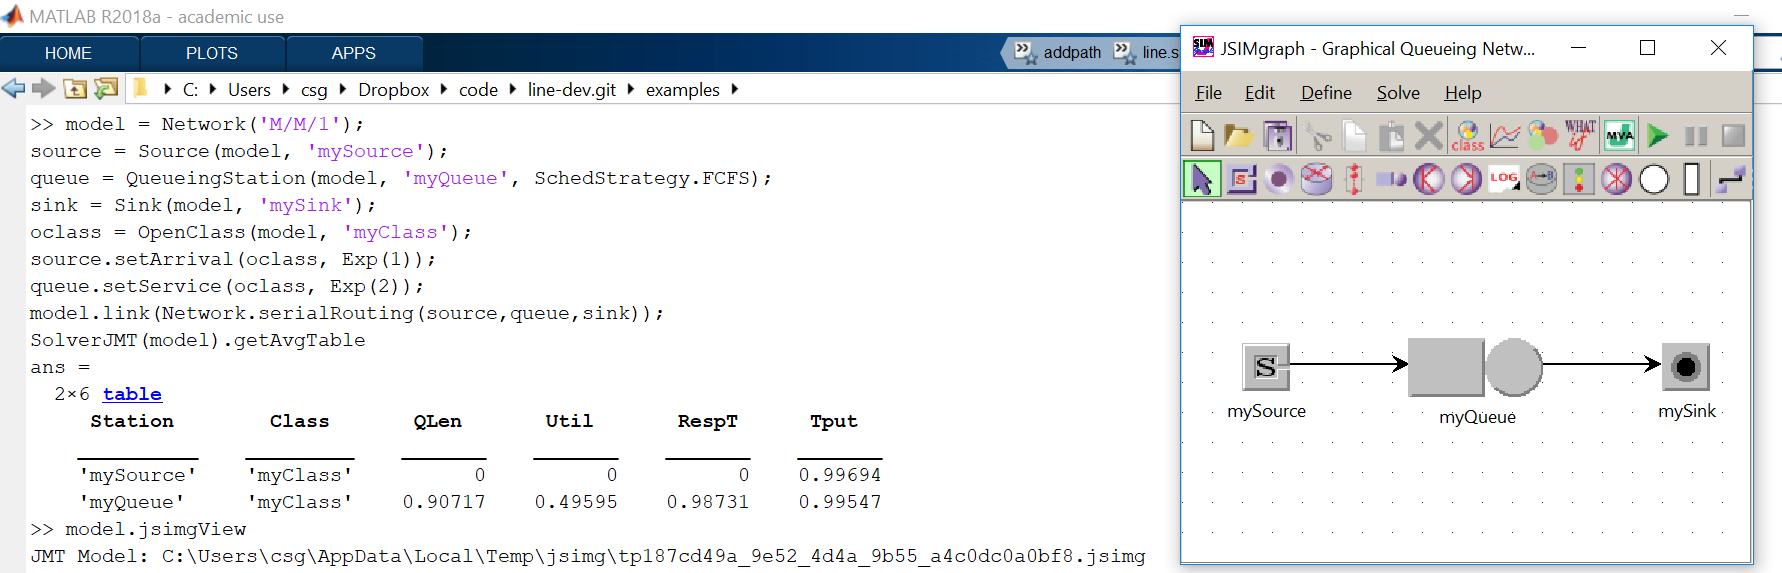
\includegraphics[width=14cm]{./images/jsimgViewMM1.png}
  \caption{M/M/1 example in JSIMgraph}\label{FIG:jsimgViewMM1}
\end{figure}

\section{Example 2: A multiclass M/G/1 queue}
\label{example-2-multiclass-mgk-queue}
We now consider a more challenging variant of the first example. We assume that there are two classes of incoming jobs with non-exponential service times. For the first class, service times are Erlang distributed with unit rate and variance $1/3$; they are instead read from a trace for the second class. Both classes have exponentially distributed service times with mean $2s$. To run this example, we assume that the reader has changed directory in MATLAB to the \texttt{examples/} folder.

We first specify the node block
\begin{lstlisting}
clear;
model = Network('M/G/1');
source = Source(model,'Source');
queue = Queue(model, 'Queue', SchedStrategy.FCFS);
sink = Sink(model,'Sink');
\end{lstlisting}
The next step consists in defining the classes. We fit automatically from mean and squared coefficient of variation (i.e., variance/mean$^2$) an Erlang distribution and use the \texttt{Replayer} distribution to request that the specified trace is cyclically read to obtain the service times of class 2
\begin{lstlisting}
jobclass1 = OpenClass(model, 'Class1');
jobclass2 = OpenClass(model, 'Class2');

source.setArrival(jobclass1, Exp(0.5));
source.setArrival(jobclass2, Exp(0.5));

queue.setService(jobclass1, Erlang.fitMeanAndSCV(1, 1/3));
queue.setService(jobclass2, Replayer('example_trace.txt'));
\end{lstlisting}
Note that the \texttt{example\_trace.txt} file consists of a single column of doubles, each representing a service time sample, e.g.,
\begin{lstlisting}
   1.2377474e-02
   4.4486055e-02
   1.0027642e-02
   2.0983173e-02
   ...
\end{lstlisting}
We now specify a linear route through source, queue, and sink for both classes
\begin{lstlisting}
P = {};
P{jobclass1} = Network.serialRouting(source,queue,sink);
P{jobclass2} = Network.serialRouting(source,queue,sink);
model.link(P);
\end{lstlisting}
and solve the model with JMT
\begin{lstlisting}
>>AvgTable = SolverJMT(model).getAvgTable
AvgTable =
  4x6 table
    Station      Class       QLen        Util       RespT      Tput
    ________    ________    _______    ________    _______    _______
    'Source'    'Class1'          0           0          0     0.5022
    'Source'    'Class2'          0           0          0    0.49999
    'Queue'     'Class1'    0.92002     0.51294     1.7724     0.5071
    'Queue'     'Class2'    0.44506    0.051639    0.85211    0.49996
\end{lstlisting}
We wish now to validate this value against an analytical solver. Since \texttt{jobclass2} has trace-based service times, we first need to revise its service time distribution to make it analytically tractable, e.g., we may ask \textsc{Line} to fit a Cox-2 distribution based on the trace
\begin{lstlisting}
queue.setService(jobclass2, Replayer('example_trace.txt').fitCox());
\end{lstlisting}
We can now use a Continuous Time Markov Chain (CTMC) to solve the system, but since the state space is infinite in open models, we need to truncate it to be able to use this solver. For example, we may restrict to states with at most 2 jobs in each class, checking with the \texttt{verbose} option the size of the resulting state space
\begin{lstlisting}
>> SolverCTMC(model,'cutoff',2,'verbose',true).getAvgTable
State space size: 46 states.
CTMC analysis completed in 0.096734 sec
ans =
  4x6 table
    Station      Class       QLen        Util       RespT      Tput
    ________    ________    _______    ________    _______    _______
    'Source'    'Class1'          0           0          0    0.44948
    'Source'    'Class2'          0           0          0    0.48424
    'Queue'     'Class1'    0.56734     0.44948     1.2863    0.44107
    'Queue'     'Class2'    0.24455    0.048942    0.51396    0.47583
\end{lstlisting}
However, we see from comparison with the JMT results that the errors are rather large. Since the truncated state space consists of just 46 states, we can further increase the cutoff to 4, trading a slower solution time for higher precision
\begin{lstlisting}
>> SolverCTMC(model,'cutoff',4,'verbose',true).getAvgTable
State space size: 626 states.
CTMC analysis completed in 1.051784 sec
ans =
  4x6 table
    Station      Class       QLen        Util       RespT      Tput
    ________    ________    _______    ________    _______    _______
    'Source'    'Class1'          0           0          0    0.49215
    'Source'    'Class2'          0           0          0    0.49626
    'Queue'     'Class1'     0.7958     0.49215     1.6187    0.49162
    'Queue'     'Class2'    0.37558    0.050157    0.75763    0.49573
\end{lstlisting}
To gain more accuracy, we could either keep increasing the cutoff value or, if we wish to compute an exact solution, we may call the matrix-analytic method (MAM) solver instead. MAM uses the repetitive structure of the CTMC to analyze exactly open systems with an infinite state space
\begin{lstlisting}
>> SolverMAM(model).getAvgTable
AvgTable =
  4x6 table
    Station      Class        QLen        Util       RespT      Tput
    ________    ________    ________    ________    _______    _______
    'Source'    'Class1'          0           0          0        0.5
    'Source'    'Class2'          0           0          0        0.5
    'Queue'     'Class1'    0.87646         0.5     1.7529        0.5
    'Queue'     'Class2'      0.427    0.050536    0.85399        0.5
\end{lstlisting}
The current \texttt{MAM} implementation is primarily constructed on top of the BuTools solver~\cite{Hor17}.

\section{Example 3: Machine interference problem}
\label{example-3-machine-interference-problem}
Closed models involve jobs that perpetually cycle within a network of queues. The machine interference problem is a classic example, in which a group of repairmen is tasked with fixing machines as they break and the goal is to choose the optimal size of the group. We here illustrate how to evaluate the performance of a given group size. We consider a scenario with two repairmen, with machines that break at a rate of $4.0$ failed machines/week, after which a machine operates as normal for an exponential distributed time with rate $0.5$ failed machines/week. There are a total of $N=3$ machines.

Suppose that we wish to obtain an exact numerical solution using Continuous Time Markov Chains (CTMCs). The above model can be analyzed as follows:
\begin{lstlisting}
model = Network('MIP');
% Block 1: nodes
delay = Delay(model,'WorkingState');
queue = Queue(model, 'RepairQueue', SchedStrategy.FCFS);
queue.setNumberOfServers(2);
% Block 2: classes
cclass = ClosedClass(model, 'Machines', 3, delay);
delay.setService(cclass, Exp(0.5));
queue.setService(cclass, Exp(4.0));
% Block 3: topology
model.link(Network.serialRouting(delay,queue));
% Block 4: solution
SolverCTMC(model,'keep',true).getAvgTable
\end{lstlisting}
Here, \texttt{delay} appears in the constructor of the closed class to specify that a machine fixing job will be considered completed once it returns to the delay (i.e., the machine is in working state). We say that the delay is thus the \emph{reference station} of class \texttt{cclass}. The above code prints the following result
\begin{lstlisting}
ans =
  2x6 table
       Station          Class        QLen       Util       RespT      Tput
    ______________    __________    _______    _______    _______    ______
    'WorkingState'    'Machines'     2.6648     2.6648          2    1.3324
    'RepairQueue'     'Machines'    0.33516    0.16655    0.25154    1.3324
\end{lstlisting}
As before, we can inspect and analyze the model in JSIMgraph using the command
\begin{lstlisting}
model.jsimgView
\end{lstlisting}
Figure~\ref{FIG:jsimgViewFRP} illustrates the result, demonstrating the automated definition of the closed class.
\begin{figure}[h!t]
  \centering
  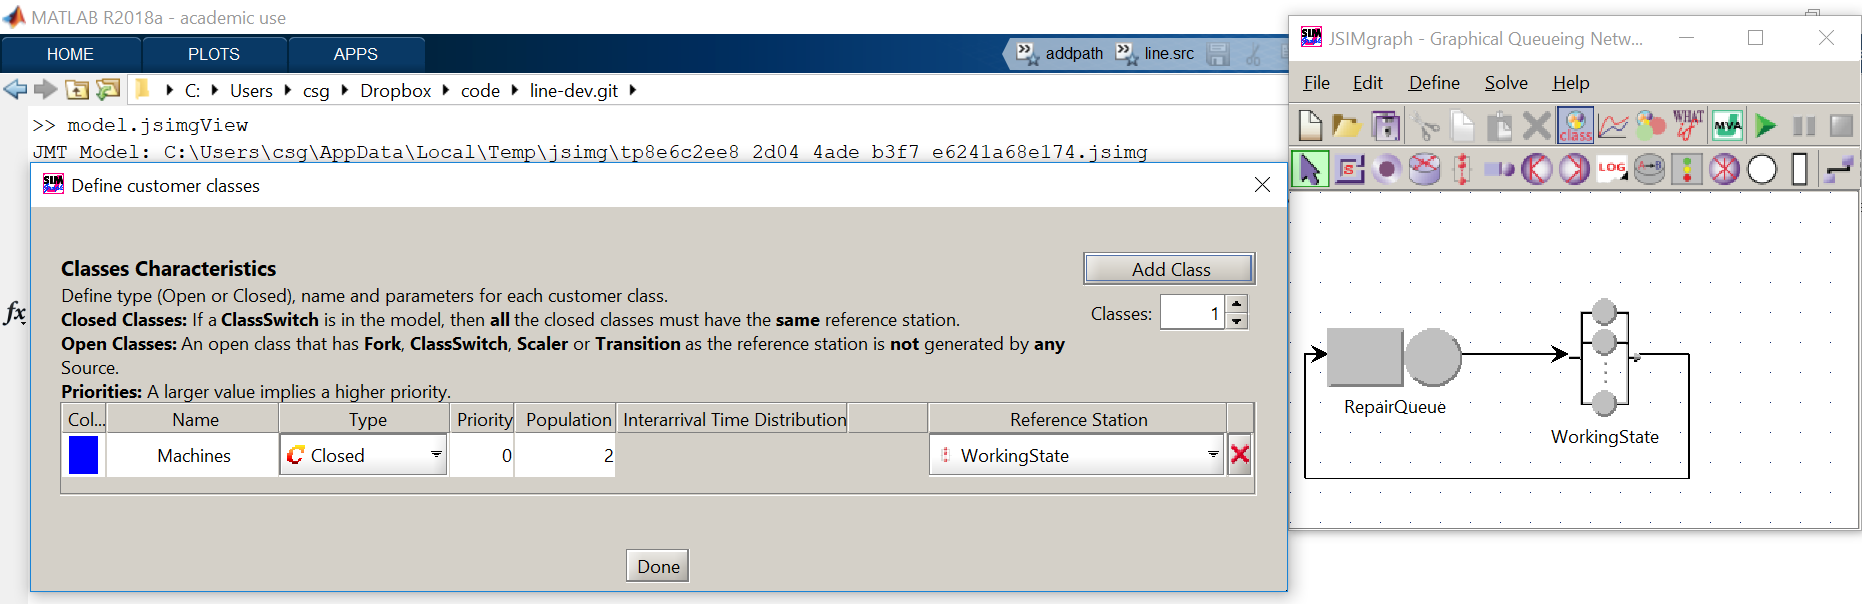
\includegraphics[width=14cm]{./images/jsimgViewFRP.png}
  \caption{Machine interference model in JSIMgraph}\label{FIG:jsimgViewFRP}
\end{figure}

The \texttt{'keep'} option we have used further allows us to inspect the infinitesimal generator of the CTMC. To do so, we retrieve some global variables that have been stored by the CTMC solver, i.e.:
\begin{lstlisting}
global InfGen;
global StateSpace;
StateSpace
InfGen=full(InfGen)
\end{lstlisting}
which produces in output the state space of the model and the infinitesimal generator of the CTMC
\begin{lstlisting}
StateSpace =
     0     1     2
     1     0     2
     2     0     1
     3     0     0
InfGen =
   -8.0000    8.0000         0         0
    0.5000   -8.5000    8.0000         0
         0    1.0000   -5.0000    4.0000
         0         0    1.5000   -1.5000
\end{lstlisting}
For example, the first state (\texttt{0 1 2}) consists of two components: the \texttt{0} is the number of jobs in service in the \texttt{delay}, while the remaining part is the state of the FCFS \texttt{queue}. In the latter, the \texttt{1} means that a job of class 1 (the only class in this model) is in the waiting buffer, while the \texttt{2} means that there are two jobs in service at the \texttt{queue}.

The second state (\texttt{1 0 2}) is similar, but one job has completed at the {queue} and then moved to the \texttt{delay}, concurrently triggering an admission in service for the job that was in the queue buffer. As a result of this, the buffer is now empty. The corresponding transition rate in the infinitesimal generator matrix is \texttt{InfGen(1,2)=8.0}, which sums the completion rates at the queue for each server, and where indexes 1 and 2 are the rows in \texttt{StateSpace} associated to the two states.

\section{Example 4: Round-robin load-balancing}
\label{example-4-round-robin-load-balancing}
In this example we consider a system of two parallel processor-sharing queues and we wish to study the effect of load-balancing on the average performance of an open class of jobs. We begin as usual with the node block, where we now include a special node, called the \texttt{Router}, to control the routing of jobs from the source into the queues:
\begin{lstlisting}
model = Network('RRLB');
source = Source(model, 'Source');
lb = Router(model, 'LB');
queue1 = Queue(model, 'Queue1', SchedStrategy.PS);
queue2 = Queue(model, 'Queue2', SchedStrategy.PS);
sink  = Sink(model, 'Sink');
\end{lstlisting}
We then define the class block by setting exponentially-distributed inter-arrival times and service times, e.g.,
\begin{lstlisting}
oclass = OpenClass(model, 'Class1');
source.setArrival(oclass, Exp(1));
queue1.setService(oclass, Exp(2));
queue2.setService(oclass, Exp(2));
\end{lstlisting}
We now wish to express the fact that the router applies a round-robin strategy to dispatch jobs to the queues. Since this is now a non-probabilistic routing strategy, we need to adopt a slightly different style to declare the topology. First, we indicate the connections between the nodes, using the \texttt{addLinks} function:
\begin{lstlisting}
model.addLinks([source, lb;
                lb,     queue1;
                lb,     queue2;
                queue1, sink;
                queue2, sink]);
\end{lstlisting}
At this point, all nodes are automatically configured to route jobs with equal probabilities on the outgoing links (\texttt{RoutingStrategy.RAND} policy). If we solve the model at this point, we see that the response time at the queues is around $0.66 s$.
\begin{lstlisting}
>> SolverJMT(model).getAvgTable
ans =
  3x6 table
    Station      Class       QLen       Util       RespT      Tput
    ________    ________    _______    _______    _______    _______
    'Source'    'Class1'          0          0          0     1.0178
    'Queue1'    'Class1'    0.32089    0.24179    0.65821    0.50222
    'Queue2'    'Class1'    0.32605    0.25078    0.66978    0.50161
\end{lstlisting}

After resetting the internal data structures, we can require \textsc{Line} to solve again the model using this time a round-robin policy at the router.
\begin{lstlisting}
model.reset()
lb.setRouting(oclass, RoutingStrategy.RR);
\end{lstlisting}
A representation of the model at this point is shown in Figure~\ref{FIG:jsimgViewLB}.
\begin{figure}[h!t]
  \centering
  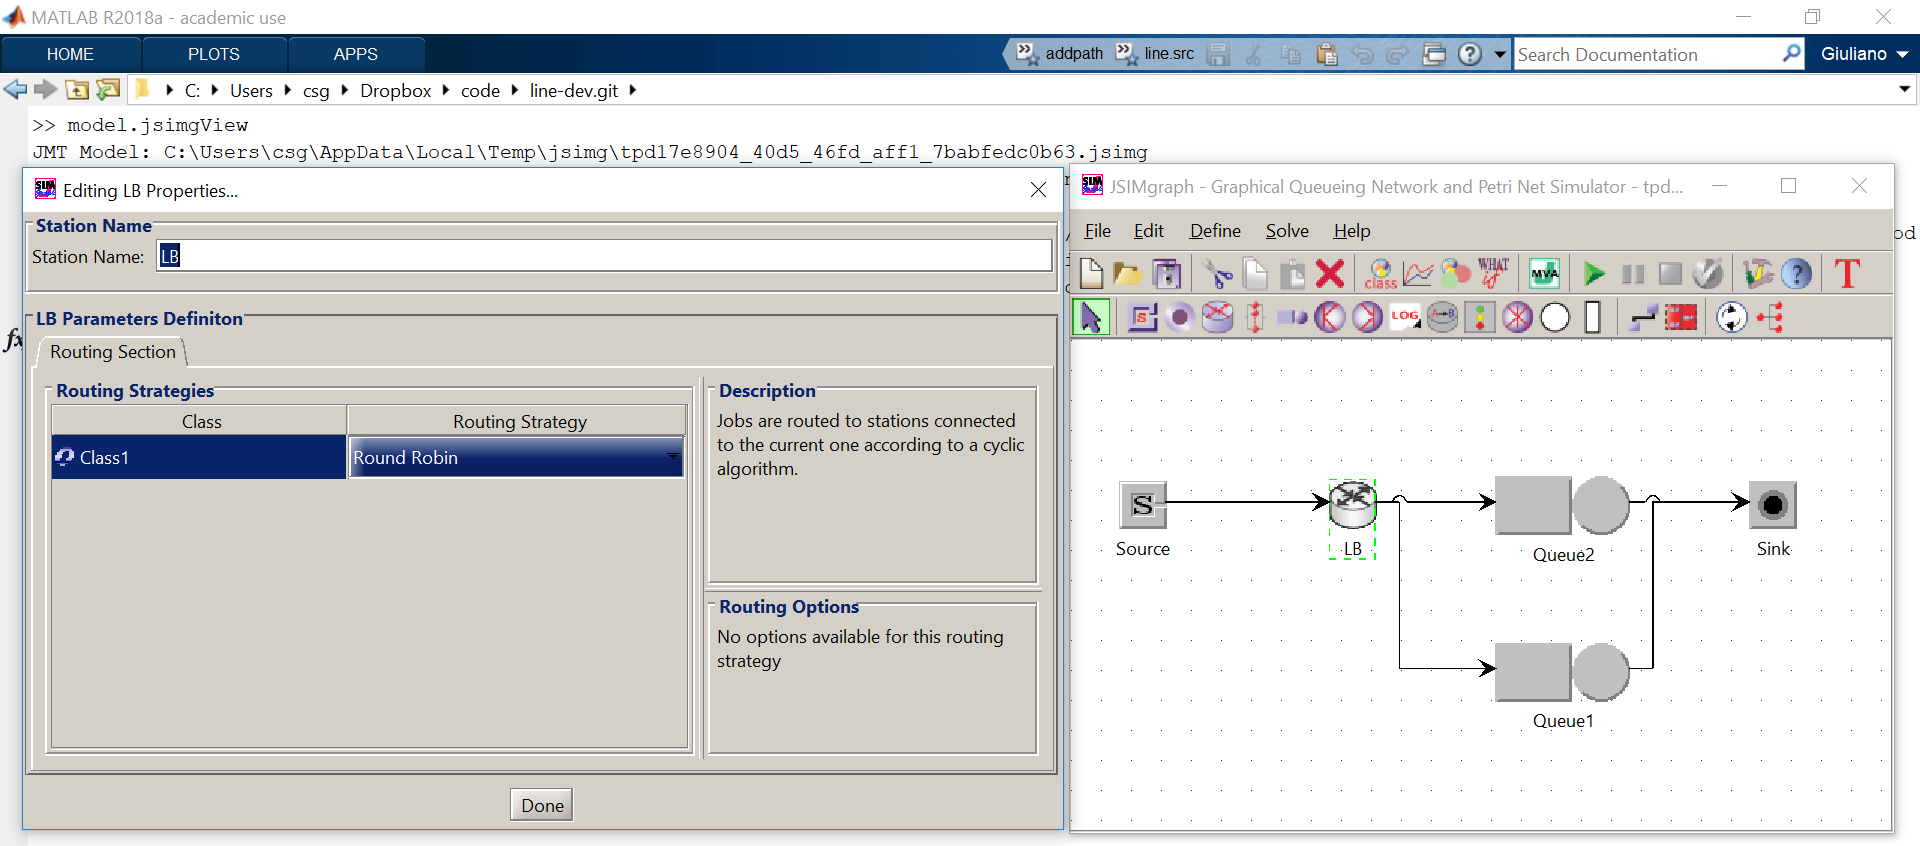
\includegraphics[width=14cm]{./images/jsimgViewLB.png}
  \caption{Load-balancing model}\label{FIG:jsimgViewLB}
\end{figure}
Lastly, we run again JMT and find that round-robin produces a visible decrease in response times
\begin{lstlisting}
>> SolverJMT(model).getAvgTable
  3x6 table
    Station      Class       QLen       Util       RespT      Tput
    ________    ________    _______    _______    _______    _______
    'Source'    'Class1'          0          0          0    0.97298
    'Queue1'    'Class1'    0.27649    0.24399    0.55775    0.48615
    'Queue2'    'Class1'    0.29316    0.24761    0.56565     0.4932
\end{lstlisting}

\section{Example 5: Modelling a re-entrant line}
\label{example-5-modelling-a-re-entrant-line}
We now consider a simple example inspired to the classic problem of modeling {\em re-entrant lines}. This arises in manufacturing systems where parts (i.e., jobs) re-enter multiple times a machine (i.e., a queueing station), asking at every visit a different class of service. This implies, for example, that the service time at every visit could feature a different mean or a different distribution, representing a different stage of processing for the part.

To illustrate this, consider for example a degenerate model composed by a single FCFS queue and $K$ classes. In this model, a job that completes processing in class $k=1,...,K$ is routed back at the tail of the queue in class $k+1$, unless $k=K$ in which case the job re-enters in class $1$.

We take the following assumptions: $K=3$; class $k$ has an Erlang-2 distribution with mean $k$; the system starts with $N_1=1$ jobs in class 1 and no jobs inside the other classes.

\begin{lstlisting}
model = Network('RL');
queue = Queue(model, 'Queue', SchedStrategy.FCFS);

K = 3; N = [1,0,0];
for k=1:K
    jobclass{k} = ClosedClass(model, ['Class',int2str(k)], N(k), queue);
    queue.setService(jobclass{k}, Erlang.fitMeanAndOrder(k,2));
end

P = cellzeros(3,3,1,1); % 3x3 cell array (3 classes) of 1x1 matrices (1 node)
P{jobclass{1},jobclass{2}}(queue,queue) = 1.0;
P{jobclass{2},jobclass{3}}(queue,queue) = 1.0;
P{jobclass{3},jobclass{1}}(queue,queue) = 1.0;
model.link(P);
\end{lstlisting}
The corresponding JMT model is shown in Figure~\ref{FIG:jsimgViewCS}, where it can be seen that the class-switching rule is automatically enforced by introduction of a \texttt{ClassSwitch} node in addition to the queue.
\begin{figure}[h!t]
  \centering
  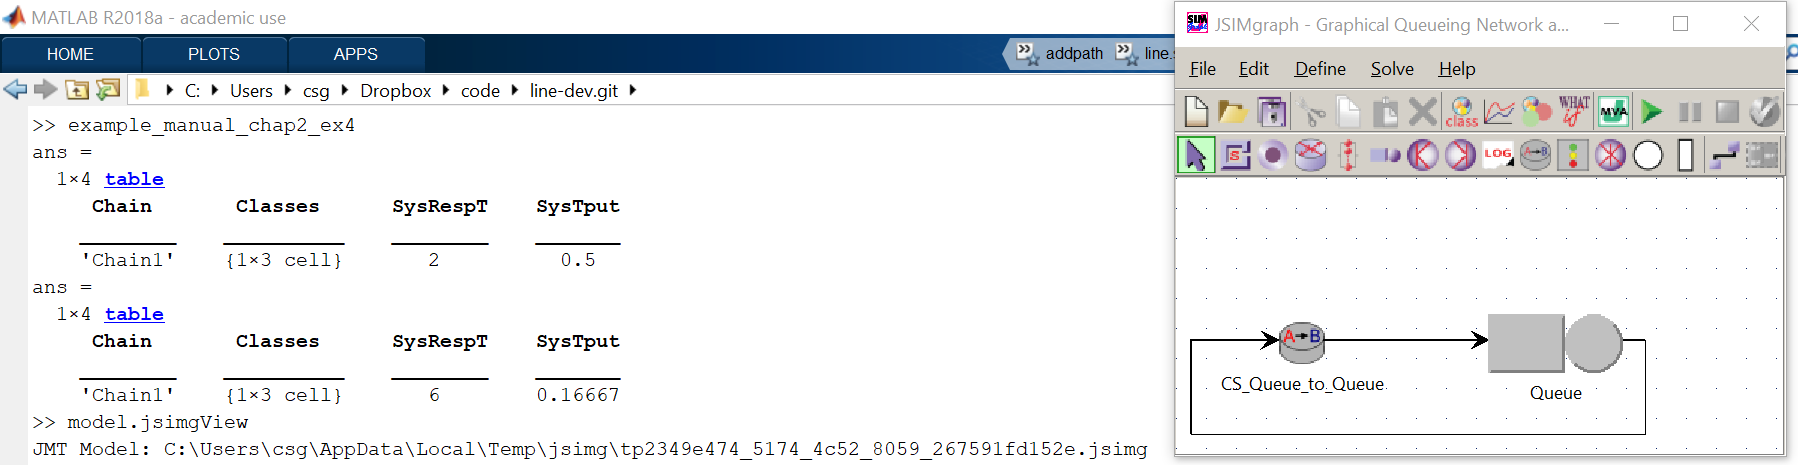
\includegraphics[width=14cm]{./images/jsimgViewCS.png}
  \caption{Re-entrant lines as an example of class-switching}
  \label{FIG:jsimgViewCS}
\end{figure}

We can now simulate the performance indexes for the different classes
\begin{lstlisting}
>> SolverCTMC(model).getAvgTable
ans =
  3x6 table
    Station     Class       QLen       Util      RespT     Tput
    _______    ________    _______    _______    _____    _______
    'Queue'    'Class1'    0.16667    0.16667      1      0.16667
    'Queue'    'Class2'    0.33333    0.33333      2      0.16667
    'Queue'    'Class3'        0.5        0.5      3      0.16667
\end{lstlisting}
Suppose now that the job is considered completed, for the sake of computation of the system's performance, only when it departs the queue in class $K$ (here \texttt{Class3}). By default, \textsc{Line} will return \emph{system-wide} performance metrics using the \texttt{getAvgSysTable} method, i.e.,
\begin{lstlisting}
>> SolverCTMC(model).getAvgSysTable
ans =
  1x4 table
     Chain       Classes      SysRespT    SysTput
    ________    __________    ________    _______
    'Chain1'    {1x3 cell}       2          0.5
\end{lstlisting}
This method identifies the model \emph{chains}, i.e., groups of classes that can exchange jobs with each other. Since the job can switch into any of the three classes, here there is a single chain comprising all three classes.

We see, however, that the throughput of this chain is $0.5$, which means that by default \textsc{Line} is counting every departure from the queue as a completion. This is because in the constructor of the closed classes, we specified \texttt{queue} as the reference station for all three classes. We could have not chosen otherwise as solution algorithms expect that all classes in a chain share the same reference station. 

To avoid this complication, we can explicitly tell to the solver that some passages through the reference station should not be counted as completions
\begin{lstlisting}
jobclass{1}.completes = false;
jobclass{2}.completes = false;
\end{lstlisting}
this then gives the correct throughput
\begin{lstlisting}
>> SolverCTMC(model).getAvgSysTable
ans =
  1x4 table
     Chain       Classes      SysRespT    SysTput
    ________    __________    ________    _______
    'Chain1'    {1x3 cell}       6        0.16667
\end{lstlisting}

\section{Example 6: A queueing network with caching}
\label{example-6-a-queueing-network-with-caching}
In this more advanced example, we show how to include in a queueing network a cache adopting a least-recently used (LRU) replacement policy. Under LRU, upon a cache miss the least-recently accessed item will be discarded to make room for the newly requested item.

We consider a cache with a capacity of 50 items, out of a set of 1000 items. Items are accessed by jobs visiting the cache according to a Zipf-like law with exponent $\alpha=1.4$ and defined over the finite set of items. A client cyclically issues requests for the items, waiting for a reply before issuing the next request. We assume that a cache hit takes on average $0.2ms$ to process, while a cache hit takes $1ms$. We ask for the average request throughput of the system, differentiated across hits and misses.

\paragraph{Node block}
As usual, we begin by defining the nodes. Here a delay node will be used to describe the time spent by the requests in the system, while the cache node will determine hits and misses:
\begin{lstlisting}
model = Network('QNC');
% Block 1: nodes
clientDelay = Delay(model, 'Client');
cacheNode = Cache(model, 'Cache', 1000, 50, ReplacementPolicy.LRU);
cacheDelay = Delay(model, 'CacheDelay');
\end{lstlisting}

\paragraph{Class block}
We define a set of classes to represent the incoming requests (\texttt{clientClass}), cache hits (\texttt{hitClass}) and cache misses (\texttt{missClass}). These classes need to be closed to ensure that there is a single outstanding request from the client at all times:
\begin{lstlisting}
% Block 2: classes
clientClass = ClosedClass(model, 'ClientClass', 1, clientDelay, 0);
hitClass = ClosedClass(model, 'HitClass', 0, clientDelay, 0);
missClass = ClosedClass(model, 'MissClass', 0, clientDelay, 0);
\end{lstlisting}
We then assign the processing times, using the \texttt{Immediate} distribution to ensure that the client issues immediately the request to the cache:
\begin{lstlisting}
clientDelay.setService(clientClass, Immediate());
cacheDelay.setService(hitClass, Exp.fitMean(0.2));
cacheDelay.setService(missClass, Exp.fitMean(1));
\end{lstlisting}
The next step involves specifying that the request uses a Zipf-like distribution to select the item to read from the cache
\begin{lstlisting}
cacheNode.setRead(clientClass, Zipf(1.4,1000));
\end{lstlisting}
Finally, we ask that the job should become of class \texttt{hitClass} after a cache hit, and should become of class \texttt{missClass} after a cache miss:
\begin{lstlisting}
cacheNode.setHitClass(clientClass, hitClass);
cacheNode.setMissClass(clientClass, missClass);
\end{lstlisting}

\paragraph{Topology block}
Next, in the topology block we setup the routing so that the request, which starts in \texttt{clientClass} at the \texttt{clientDelay}, then moves from there to the cache, remaining in \texttt{clientClass}
\begin{lstlisting}
% Block 3: topology
P = cellzeros(3,3,4,4); % 3x3 cell (3 classes) of 4x4 zero matrices (4 nodes)
P{clientClass, clientClass}(clientDelay, cacheNode) = 1.0;
\end{lstlisting}
Internally to the cache, the job will switch its class into either \texttt{hitClass} or \texttt{missClass}. Upon departure in one of these classes, we ask it to join in the same class \texttt{cacheDelay} for further processing
\begin{lstlisting}
P{hitClass, hitClass}(cacheNode, cacheDelay) = 1.0;
P{missClass, missClass}(cacheNode, cacheDelay) = 1.0;
\end{lstlisting}
Lastly, the job returns to \texttt{clientDelay} for completion and start of a new request, which is done by switching its class back to \texttt{clientClass}
\begin{lstlisting}
P{hitClass, clientClass}(cacheDelay, clientDelay) = 1.0;
P{missClass, clientClass}(cacheDelay, clientDelay) = 1.0;
\end{lstlisting}
The above routing strategy is finally applied to the model
\begin{lstlisting}
model.link(P);
\end{lstlisting}

\paragraph{Solution block}
To solve the model, since JMT does not support cache modeling, we use the native MATLAB-based simulation engine provided within \textsc{Line}, the \texttt{SSA} solver:
\begin{lstlisting}
% Block 4: solution
AvgTable = SolverSSA(model,'samples',2e4,'seed',1,'verbose',true).getAvgTable
\end{lstlisting}
The above script produces the following result
\begin{lstlisting}
SSA samples:   20000
SSA analysis completed in 11.902675 sec
AvgTable =
 3x6 table
     Station           Class         QLen       Util      RespT     Tput
   ____________    _____________    _______    _______    _____    _______
   'Client'        'ClientClass'          0          0       0      2.9917
   'CacheDelay'    'HitClass'       0.49108    0.49108     0.2      2.4554
   'CacheDelay'    'MissClass'      0.50892    0.50892       1     0.50892
\end{lstlisting}
The departing flows from the \texttt{CacheDelay} are the miss and hit rates. Thus, the hit rate is $2.4554$ req/ms, while the miss rate is $0.50892$ req/ms, which both include the service times.

Let us now suppose that we wish to verify the result with a longer simulation, for example with 10 times more samples. To this aim, we can use the automatic parallelization of \texttt{SSA} based on MATLAB's \texttt{spmd} construct:
\begin{lstlisting}
SolverSSA(model,'samples',2e4,'seed',1,'method','parallel').getAvgTable
\end{lstlisting}
This gives us a rather similar result, when run on a dual-core machine
\begin{lstlisting}
Starting parallel pool (parpool) using the 'local' profile ...
connected to 2 workers.
AvgTable =
 3x6 table
     Station           Class         QLen      Util     RespT     Tput
   ____________    _____________    ______    ______    _____    ______
   'Client'        'ClientClass'         0         0       0     2.8636
   'CacheDelay'    'HitClass'       0.4709    0.4709     0.2     2.3545
   'CacheDelay'    'MissClass'      0.5291    0.5291       1     0.5291
\end{lstlisting}
The execution time is longer than usual at the first invocation of the parallel solver due to the time needed by MATLAB to bootstrap the parallel pool, in this example around 22 seconds. Successive invocations of parallel SSA normally take much less, with this example around 7 seconds each.

%\section{Example 4: Server breakdown and repair}

%\section{Example 5: A two-layer network}


\chapter{Network models}
\label{Network-models}

Throughout this chapter, we discuss the specification of \texttt{Network} models. %Instead, we point to the following chapters for \texttt{CacheNetwork} and \texttt{LayeredNetwork} models.
It is important to keep in mind that not all of the model features described in the present chapter are supported by every
\textsc{Line} solver. However, upon calling a solver, \textsc{Line} will automatically detect if the supplied model can be
analyzed by that solver and return an empty set if not. Tables are given later in the manual summarizing the features supported by each solver.

\section{Network object definition}
\label{network-object-definition}
\subsection{Creating a network and its nodes}
A queueing network can be described in \textsc{Line} using the \texttt{Network} class constructor with a unique string identifying the model name:
\begin{lstlisting}
model = Network('myModel');
\end{lstlisting}
The returned object of the \texttt{Network} class offers functions to instantiate and manage resource \emph{nodes} (stations,  delays, caches, ...) visited by jobs of several types (\emph{classes}).

A {node} is a resource in the network that can be visited by a job. A node must have a unique name and can either be {\em stateful} or {\em stateless}, the latter meaning that the node does not require state variables to determine the actions it performs on the system. If jobs visiting a stateful node can be required to spend time in it, the node is also said to be a {\em station}. A list of nodes available in \texttt{Network} models is given in the next table.

\begin{table}[h!]
\caption{Nodes available in \texttt{Network} models.}
\begin{tabular}{|l|l|p{9.7cm}|}
\hline
{Node} & {Type} & {Description} \\
\hline
\texttt{Cache} & stateful node & A class-switching router based on cache hits/misses\\
\texttt{ClassSwitch} & stateless node & A class-switching router based on a static probability matrix\\
\texttt{Delay} & station & A station where jobs spend time without queueing\\
%\texttt{Logger} & stateless node & A node that logs passage of jobs\\
\texttt{Queue} & station & A generic queueing element\\
%\texttt{Router} & stateful node & A node that routes jobs\\
\texttt{Sink} & stateless node & Exit point for jobs in open classes\\
\texttt{Source} & station & Entry point for jobs in open classes\\
\hline
\end{tabular}
\end{table}

For example, a sink is a stateless node, since its behaviour does not require state variables and jobs cannot sojourn in it. Instead, a first-come first-served queue is a station, since jobs can sojourn inside its buffer and servers. A source is also treated in \textsc{Line} as a station since the inter-arrival time of jobs from the external world is considered as a time spent in the source, although this is not counted as part of the system response time.
Lastly, a cache is a stateful node, since it needs to keep track of the cached items, however it is not a station since passage through this node occurs instantaneously.

We now provide more details on each of the nodes available in \texttt{Network} models.
\paragraph{Queue node.}
Among the listed nodes, the most important one is the \texttt{Queue}, which specifies a queueing station from its name and scheduling strategy, e.g.
\begin{lstlisting}
queue = Queue(model, 'Queue1', SchedStrategy.FCFS);
\end{lstlisting}
It is also possible to instantiate a queue using the \texttt{QueueingStation} constructor, which is merely an alias for the \texttt{Queue} class.

Valid scheduling strategies are specified within the \texttt{SchedStrategy} static class and include:
\begin{itemize}
\item First-come first-served (\texttt{SchedStrategy.FCFS})
\item Infinite-server (\texttt{SchedStrategy.INF})
\item Processor-sharing (\texttt{SchedStrategy.PS})
\item Discriminatory processor-sharing (\texttt{SchedStrategy.DPS})
\item Generalized processor-sharing (\texttt{SchedStrategy.GPS})
\item Shortest expected processing time (\texttt{SchedStrategy.SEPT})
\item Shortest job first (\texttt{SchedStrategy.SJF})
\item Head-of-line priority (\texttt{SchedStrategy.HOL})
\end{itemize}
If a strategy requires class weights, these can be specified directly as an argument to the \texttt{setService} function or using the \texttt{setStrategyParam} function, see later the description of DPS scheduling for an example.

\paragraph{Delay node.} Infinite-server stations may be instantiated either as objects of \texttt{Queue} class with the \texttt{SchedStrategy.INF} strategy or using the following specialized constructor
\begin{lstlisting}
delay = Delay(model, 'ThinkTime');
\end{lstlisting}
As for queues, for readability it is possible to instantiate delay nodes using the \texttt{DelayStation} constructor, which is entirely equivalent to the one of the \texttt{Delay} class.

\paragraph{Source and Sink nodes.} As seen in the M/M/1 getting started example, these nodes are mandatory elements for the specification of open classes. Their constructor only requires a specification of the unique name associated to the nodes:
\begin{lstlisting}
source = Source(model, 'Source');
sink = Sink(model, 'Sink');
\end{lstlisting}

\paragraph{ClassSwitch node.} This is a stateless node to change the class of a transiting job based on a static probabilistic policy. For example, it is possible to specify that all jobs belonging to class 1 should become of class 2, or that a class 2 job should become of class 1 with probability $0.3$. This example is instantiated as follows
\begin{lstlisting}
cs = ClassSwitch(model, 'ClassSwitchPoint',[0.0, 1.0; 0.3, 0.7]);
\end{lstlisting}

\paragraph{Cache node.} This is a stateful node to store one or more items in a cache of finite size, for which it is possible to specify a replacement policy.  The cache constructor requires the total cache capacity and the number of items that can be referenced by the jobs in transit, e.g.,
\begin{lstlisting}
cacheNode = Cache(model, 'Cache1', nitems, capacity, ReplacementPolicy.LRU);
\end{lstlisting}
If the capacity is an integer (e.g., \texttt{[15]}) , then it represents the total number of items that can be cached and the value cannot be greater than the number of items. Conversely, if it is a vector (e.g., \texttt{[10,5]}) then the node is a list-based cache, where the vector entries specify the capacity of each list. We point to \cite{GastH16} for more details on list-based caches and their replacement policies.

Available replacement policies are specified within the \texttt{ReplacementPolicy} static class and include:
\begin{itemize}
\item First-in first-out (\texttt{ReplacementPolicy.FIFO})
\item Random replacement (\texttt{ReplacementPolicy.RAND})
\item Least-recently used (\texttt{ReplacementPolicy.LRU})
\item Strict first-in first-out (\texttt{ReplacementPolicy.SFIFO})
\end{itemize}
Upon cache hit or cache miss, a job in transit is switched to a user-specified class. More details are given later in Section~\ref{class-switching}.

\subsection{Job classes}
Jobs travel within the network placing service demands at the stations. The demand placed by a job at a station depends on the class of the job. Jobs in {\em open classes} arrive from the external world and, upon completing the visit, leave the network. Jobs in {\em closed classes} start within the network and are forbidden to ever leave it, perpetually cycling among the nodes.

\subsubsection{Open classes}
The constructor for an open class only requires the class name and the creation of special nodes called \texttt{Source} and \texttt{Sink}
\begin{lstlisting}
source = Source(model, 'Source');
sink = Sink(model, 'Sink');
\end{lstlisting}
Sources are special stations holding an infinite pool of jobs and representing the external world. Sinks are nodes that route a departing job back into this infinite pool, i.e., into the source. Note that a network can include at most a single \texttt{Source} and a single \texttt{Sink}.

Once source and sink are instantiated in the model, it is possible to instantiate open classes using
\begin{lstlisting}
class1 = OpenClass(model, 'Class1');
\end{lstlisting}
\textsc{Line} does not require to associate source and sink with the open classes in their constructors, as this is done automatically. However, the \textsc{Line} language requires to explicitly create these nodes since the routing topology needs to indicate the arrival and departure points of jobs in open classes. However, if the network does not includes open classes, the user will not need to instantiate a \texttt{Source} and a \texttt{Sink}.

\subsubsection{Closed classes}
To create a closed class, we need instead to indicate the number of jobs that start in that class (e.g., 5 jobs) and the {\em reference station} for that class (e.g., \texttt{queue}), i.e.:
\begin{lstlisting}
class2 = ClosedClass(model, 'Class2', 5, queue);
\end{lstlisting}
The reference station indicates a point in the network used to calculate certain performance indexes, called {\em system performance indexes}. The end-to-end response time for a job in an open class to traverse the system is an example of system performance index (system response time). The reference station of an open class is always automatically set by \textsc{Line} to be the \texttt{Source}. Conversely the reference station needs to be indicated explicitly in the constructor for closed classes, since the point at which a class job completes execution depends on the semantics of the model.

\subsubsection{Mixed models}
\textsc{Line} also accepts models where a user has instantiated both open and closed classes. The only requirement is that, if two classes communicate by means of a class-switching mechanism, then the two classes must either be all closed or all open. In other words, classes in the same chain must either be both closed or both open. Furthermore, for closed classes in the same chain it is required that the reference station is the same.

\subsubsection{Class priorities}
If a class has a priority, with 0 representing the highest priority, this can be specified as an additional argument to both \texttt{OpenClass} and \texttt{ClosedClass}, e.g.,
\begin{lstlisting}
class2 = ClosedClass(model, 'Class2', 5, queue, 0);
\end{lstlisting}
In \texttt{Network} models, priorities are intended as hard priorities and the only supported priority scheduling strategy (\texttt{SchedStrategy.HOL}) is non-preemptive. Weight-based policies such as DPS and GPS may be used, as an alternative, to prevent starvation of jobs in low priority classes.

\subsection{Routing strategies}
\subsubsection{Probabilistic routing}
Jobs travel between nodes according to the network topology and a routing strategy. Typically a queueing network will use a probabilistic routing strategy (\texttt{RoutingStrategy.PROB}), which requires to specify routing probabilities among the nodes. The simplest way to specify a large routing topology is to define the routing probability matrix for each class, followed by a call to the \texttt{link} function. This function will automatically add certain nodes to the network to ensure the correct switching of class for jobs moving between stations (\texttt{ClassSwitch} elements).

In the running case, we may instantiate a routing topology as follows:
\begin{lstlisting}
P = cellzeros(2,4);
P{class1}(source,queue) = 1.0;
P{class1}(queue,[queue,delay]) = [0.3,0.7]; % self-loop with probability 0.3
P{class1}(delay,sink) = 1.0;
P{class2}(delay,queue) = 1.0; % closed class starts at delay
P{class2}(queue,delay) = 1.0;
model.link(P);
\end{lstlisting}
When used as arguments to a cell array or matrix, class and node objects will be replaced by a corresponding numerical index.
Normally, the indexing of classes and nodes matches the order in which they are instantiated in the model and one can therefore specify the routing matrices using this property. In this case we would have
\begin{lstlisting}
P = cellzeros(2,4);
P{class1} = [0,1,0,0;   % row: source
             0,.3,.7,0; % row: queue
             0,0,0,1;   % row: delay
             0,0,0,0];  % row: sink
P{class2} = [0,0,0,0;
             0,0,1,0;
             0,1,0,0;
             0,0,0,0];
model.link(P);
\end{lstlisting}
The \texttt{getClassIndex} and \texttt{getNodeIndex} functions return the numerical index associated to a node name, e.g.,
\texttt{model.getNodeIndex('Delay')}. Class and node names in a network need to be unique. The list of used names can be obtained with the \texttt{getClassNames}, \texttt{getStationNames}, and \texttt{getNodeNames} functions of the \texttt{Network} class.

It is also important to note that the routing matrix in the last example is specified between {\em nodes}, instead than between just stations or stateful nodes, which means that elements such as the \texttt{Sink} need to be explicitly considered in the routing matrix. The only exception is that \texttt{ClassSwitch} elements do not need to be explicitly instantiated and explicited in the routing matrix, provided that one uses the \texttt{link} function to instantiate the topology. Note that the routing matrix assigned to a model can be printed on screen in human-readable format using the \texttt{printRoutingMatrix} function.

\subsubsection{Other routing strategies}
The above routing specification style is only for models with probabilistic routing strategies between every pair of nodes. A different style should be used for scheduling policies that do not require to explicit routing probabilities, as in the case of state-dependent routing. Currently supported strategies include:
\begin{itemize}
\item Round robin (\texttt{RoutingStrategy.RR}). This is a non-probabilistic strategy that sends jobs to outgoing links in a cyclic order. %It is currently supported only by \texttt{SolverJMT}.
\item Random routing (\texttt{RoutingStrategy.RAND}). This is equivalent to a standard probabilistic strategy that for each class assigns identical values to the routing probabilities of all outgoing links.
\item Join-the-Shortest-Queue (\texttt{RoutingStrategy.JSQ}).  This is a non-probabilistic strategy that sends jobs to the destination with the smallest total number of jobs in it. If multiple stations have the same total number of jobs, then the destination is chosen at random with equal probability across these stations.
\end{itemize}
For such policies, the function \texttt{addLink} should be first used to specify pairs of connected nodes
\begin{lstlisting}
model.addLink(queue, queue); %self-loop
model.addLink(queue, delay);
\end{lstlisting}
Then an appropriate routing strategy should be selected at every node, e.g.,
\begin{lstlisting}
queue.setRouting(class1,RoutingStrategy.RR);
\end{lstlisting}
assigns round robin among all outgoing links from the \texttt{queue} node.

A model could also include both classes with probabilistic routing strategies and classes that use round robin or other non-probabilistic startegies. To instantiate routing probabilities in such situations one should then use, e.g.,
\begin{lstlisting}
queue.setRouting(class1,RoutingStrategy.PROB);
queue.setProbRouting(class1, queue, 0.7)
queue.setProbRouting(class1, delay, 0.3)
\end{lstlisting}
where \texttt{setProbRouting} assigns the routing probabilities to the two links.

\subsection{Class switching}
\label{class-switching}

In \textsc{Line}, jobs can switch class while they travel between nodes (including self-loops on the same node). For example, this feature can be used to model queueing properties such as re-entrant lines in which a job visiting a station a second time may require a different average service demand than at its first visit.

A chain defines the set of reachable classes for a job that starts in the given class $r$ and over time changes class. Since class switching in \textsc{Line} does not allow a closed class to become open, and vice-versa, chains can themselves be classified into {\em open chains} and {\em closed chains}, depending on the classes that compose them.

Jobs in open classes can only switch to another open class. Similarly, jobs in closed classes can only switch to a closed class. Thus, class switching from open to closed classes (or vice-versa) is forbidden. The strategy to describe the class switching mechanism is integrated in the specification of the routing between stations as described next.

\subsubsection{Probabilistic class switching}
In models with class switching and probabilistic routing at all nodes, a routing matrix is required for each possible pair of source and target classes. For example, suppose that in the previous example the job in the closed class \texttt{class2} switches into a new closed class (\texttt{class3}) while visiting the \texttt{queue} node. We can specify this routing strategy as follows:
\begin{lstlisting}
class3 = ClosedClass(model, 'Class3', 0, queue, 0);

P = cellzeros(3,3,4);
P{class1,class1}(source, queue) = 1.0;
P{class1,class1}(queue, [queue,delay]) = [0.3,0.7];
P{class1,class1}(delay, sink) = 1.0;
P{class2,class3}(delay, queue) = 1.0; % closed class starts at delay
P{class3,class2}(queue, delay) = 1.0;
model.link(P);
\end{lstlisting}
where \texttt{P\{r,s\}} is the routing matrix for jobs switching from class \texttt{r} to \texttt{s}. That is, \texttt{P\{r,s\}(i,j)} is the probability that a job in class \texttt{r} departs node \texttt{i} routing into node \texttt{j} as a job of class \texttt{s}.

Importantly, \textsc{Line} assumes that a job switches class an instant {\em after} leaving a station, thus the performance metrics of a class at the node refer to the class that jobs had upon arrival to that node.

Depending on the specified probabilities, a job will be able to switch class only among a subset of the available classes. Each subset is called a {\em chain}. Chains are computed in \textsc{Line} as the weakly connected components of the routing probability matrix of the network, when this is seen as an undirected graph. The function \texttt{model.getChains} produces the list of chains for the model, inclusive of a list of their composing classes.

An advanced feature of \textsc{Line} available for example within the \texttt{Cache} node, is that the class-switching decision can dynamically depend on the state of the node (e.g., cache hit/cache miss). However, in order to statically determine chains, \textsc{Line} requires that every class-switching node declares the pair of classes that can potentially communicate with each other via a switch. This is called the {\em class-switching mask} and it is automatically computed. The boolean matrix returned by the \texttt{model.getClassSwitchingMask} function provides this mask, which has entry in row $r$ and column $s$ set to true only if jobs in class $r$ can switch into class $s$ at some node in the network.

\subsubsection{Class switching with non-probabilistic routing strategies}
In the presence of non-probabilistic routing strategies, one needs to specify more details of the class switching mechanism. This can be done through addition to the network topology of \texttt{ClassSwitch} elements. The constructor of this node requires to specify a probability matrix $C$ such that $C(r,s)$ is the probability that a job of class $r$ arriving into the \texttt{ClassSwitch} switches to class $s$ during the visit. For example, in a 2-class model the following node will switch all visiting jobs into class 2
\begin{lstlisting}
C = [0, 1; 0, 1];
node = ClassSwitch(model, 'CSNode',C);
\end{lstlisting}
Note that for a network with $M$ stations, up to $M^2$ \texttt{ClassSwitch} elements may be required to implement class-switching across all possible links, including self-loops. Moreover, refreshing network parameters under non-probabilistic routing strategies may .

Contrary to the \texttt{link} function, one cannot specify in the argument to \texttt{setProbRouting} a class switching probability. The \texttt{setProbRouting} function should instead be used to route the job through an appropriate \texttt{ClassSwitch} element.

\subsubsection{Routing probabilities for Source and Sink nodes}
In the presence of open classes, and in mixed models with both open and closed classes, one needs only to specify the routing probabilities {\em out} of the source. The probabilities out of the sink can all be set to zero for all classes and destinations (including self-loops). The solver will take care of adjusting these inputs to create a valid routing table.

\subsubsection{Cache-based class-switching}
\label{cache-based-class-switching}
Upon cache hit or cache miss, a job in transit is switched to a user-specified class, as specified by the \texttt{setHitClass} and \texttt{setMissClass}, so that it can be routed to a different destination based on wether it found the item in the cache or not. The \texttt{setRead} function allows the user to specify a discrete distribution (e.g., \texttt{Zipf}, \texttt{DiscreteDistrib}) for the frequency at which an item is requested. For example,
\begin{lstlisting}
refModel = Zipf(0.5,nitems);
cacheNode.setRead(initClass, refModel);
cacheNode.setHitClass(initClass, hitClass);
cacheNode.setMissClass(initClass, missClass);
\end{lstlisting}
Here \texttt{initClass}, \texttt{hitClass}, and \texttt{missClass} can be either open or closed instantiated as usual with the \texttt{OpenClass} or \texttt{ClosedClass} constructors.

\subsubsection{Reference station}
\label{reference-station}
Before we have shown that the specification of classes requires to choose a reference station. In \textsc{Line}, reference stations are properties of chains, thus if two closed classes belong to the same chain they must have the same reference station. This avoids ambiguities in the definition of the completion point for jobs within a chain.

For example, the system throughput for a chain is defined as sum of the arrival rates at the reference station for all classes in that chain. That is, the solver counts a return to the reference station as a completion of the visit to the system. In the case of open chains, the reference station is always the \texttt{Source} and the system throuhput corresponds to the rate at which jobs arrive to the sink \texttt{Sink}, which may be seen as the arrival rate seen by the infinite pool of jobs in the external world. If there is no class switching, each chain contain a single class, thus per-chain and per-class performance indexes will be identical.


\subsubsection{Tandem and cyclic topologies}
Tandem networks are open queueing networks with a serial topology. \textsc{Line} provides functions that ease the definition of tandem networks of stations with exponential service times. For example, we can rapidly instantiate a tandem network consisting of stations with PS and INF scheduling as follows
\begin{lstlisting}
A = [10,20]; % A(r) - arrival rate of class r
D = [11,12; 21,22]; % D(i,r) - class-r demand at station i (PS)
Z = [91,92; 93,94]; % Z(i,r)  - class-r demand at station i (INF)
modelPsInf = Network.tandemPsInf(A,D,Z)
\end{lstlisting}
The above snippet instantiates an open network with two queueing stations (PS), two delay stations (INF), and exponential distributions with the given inter-arrival rates and mean service times. The \texttt{Network.tandemPs}, \texttt{Network.tandemFcfs}, and \texttt{Network.tandemFcfsInf} functions provide static constructors for networks with other combinations of scheduling policies, namely only PS, only FCFS, or FCFS and INF.

A tandem network with closed classes is instead called a cyclic network. Similar to tandem networks, \textsc{Line} offers a set of static constructors: \texttt{Network.cyclicPs}, \texttt{Network.cyclicPsInf}, \texttt{Network.cyclicFcfs}, and \texttt{Network.cyclicFcfsInf}. These functions only require to replace the arrival rate vector \texttt{A} by a vector \texttt{N} specifying the job populations for each of the closed classes, e.g.,
\begin{lstlisting}
N = [10,20]; % N(r) - closed population in class r
D = [11,12; 21,22]; % D(i,r) - class-r demand at station i (PS)
modelPsInf = Network.cyclicPs(N,D)
\end{lstlisting}

\subsection{Finite buffers}
The functions \texttt{setCapacity} and \texttt{setChainCapacity} of the \texttt{Station} class are used to place constraints on the number of jobs, total or for each chain, that can reside within a station. Note that \textsc{Line} does not allow one to specify buffer constraints at the level of individual classes, unless chains contain a single class, in which case \texttt{setChainCapacity} is sufficient for the purpose.

For example,
\begin{lstlisting}
example_closedModel_3
delay.setChainCapacity([1,1])
model.refreshCapacity()
\end{lstlisting}
creates an example model with two chains and three classes (specified in \texttt{example\_closedModel\_3.m}) and requires the second station to accept a maximum of one job in each chain. Note that if we were to ask for a higher capacity, such as \texttt{setChainCapacity([1,7])}, which exceeds the total job population in chain 2, \textsc{Line} would have automatically reduced the value 7 to the chain 2 job population (2). This automatic correction ensures that functions that analyze the state space of the model do not generate unreachable states.

The \texttt{refreshCapacity} function updates the buffer parameterizations, performing appropriate sanity checks. Since \texttt{example\_closedModel\_3} has already invoked a solver prior to our changes, the requested modifications are materially applied by \textsc{Line} to the network only after calling an appropriate \texttt{refreshStruct} function, see the sensitivity analysis section. If the buffer capacity changes were made before the first solver invocation on the model, then there would not be need for a \texttt{refreshCapacity} call, since the internal representation of the \texttt{Network} object used by the solvers is still to be created.

\subsection{Service and inter-arrival time processes}
\label{service-and-inter-arrival-time-processes}
A number of statistical distributions are available to specify job service times at the stations and inter-arrival times from the \texttt{Source} station. The class \texttt{PhaseType} offers distributions that are analytically tractable, which are defined upon certain absorbing Markov chains consisting of one or more states ({\em phases}) that are called phase-type distributions. They include as special case the following distributions supported in \textsc{Line}, along with their respective constructors:
\begin{itemize}
\item Exponential distribution: \texttt{Exp}$(\lambda)$, where $\lambda$ is the rate of the exponential
\item $n$-phase Erlang distribution: \texttt{Erlang}$(\alpha, n)$, where $\alpha$ is the rate of each of the $n$ exponential phases
\item $2$-phase hyper-exponential distribution: \texttt{HyperExp}$(p,\lambda_1,\lambda_2)$, that returns an exponential with rate $\lambda_1$ with probability $p$, and  an exponential with rate $\lambda_2$ otherwise.
\item $2$-phase Coxian distribution: \texttt{Cox2}$(\mu_1,\mu_2,\phi_1)$, which assigns rates $\mu_1$ and $\mu_2$ to the two rates, and completion probability from phase 1 equal to $\phi_1$ (the probability from phase 2 is $\phi_2=1.0$).
\end{itemize}
For example, given mean $\mu=0.2$ and squared coefficient of variation SCV=10, where SCV=variance/$\mu^2$, we can assign to a node a $2$-phase Coxian service time distribution with these moments as
\begin{lstlisting}
queue.setService(class2, Cox2.fitMeanAndSCV(0.2,10));
\end{lstlisting}
Inter-arrival time distributions can be instantiated in a similar way, using \texttt{setArrival} instead of \texttt{setService} on the \texttt{Source} node. For example, if the \texttt{Source} is node 3 we may assign the inter-arrival times of class 2 to be exponential with mean 0.1 as follows
\begin{lstlisting}
source.setArrival(class2, Exp.fitMeanAndSCV(0.1));
\end{lstlisting}
where we have used a single parameter in \texttt{fitMeanAndSCV} since the exponential distribution does not allow to choose the SCV.

Non-Markovian distributions are also available, but typically they restrict the available network analysis techniques to simulation. They include the following distributions:
\begin{itemize}
\item Deterministic distribution: \texttt{Det}$(\mu)$ assigns probability 1.0 to the value $\mu$.
\item Uniform distribution: \texttt{Uniform}$(a,b)$ assigns uniform probability $1/(b-a)$ to the interval $[a,b]$.
\item Gamma distribution: \texttt{Gamma}$(\alpha, k)$ assigns a gamma density with shape $\alpha$ and scale $k$.
\item Pareto distribution: \texttt{Pareto}$(\alpha, k)$ assigns a Pareto density with shape $\alpha$ and scale $k$.
\end{itemize}

Lastly, we discuss two special distributions. The \texttt{Disabled} distribution can be used to explicitly forbid a class to receive service at a station. This may be useful in models with sparse routing matrices, both to ensure an efficient model solution and to debug the model specification. Performance metrics for disabled classes will be set to \texttt{NaN}.

Conversely, the \texttt{Immediate} class can be used to specify instantaneous service (zero service time). Typically, \textsc{Line} solvers will replace zero service times with small positive values ($\varepsilon=10^{-7}$).

\subsubsection{Fitting a distribution}
The \texttt{fitMeanAndSCV} function is available for all distributions that inherit from the \texttt{PhaseType} class. This function provides exact or approximate matching of the requested moments, depending on the theoretical constraints imposed by the distribution. For example, an Erlang distribution with SCV=0.75 does not exist, because in a $n$-phase Erlang it must be SCV=$1/n$. In a case like this, \texttt{Erlang.fitMeanAndSCV(1,0.75)} will return the closest approximation, e.g., a 2-phase Erlang (SCV=0.5) with unit mean. The Erlang distribution also offer a function \texttt{fitMeanAndOrder}$(\mu,n)$, which instantiates a $n$-phase Erlang with given mean $\mu$.

In distributions that are uniquely determined by more than two moments, \texttt{fitMeanAndSCV} chooses a particular assignment of the residual degrees of freedom other than mean and SCV. For example, \texttt{HyperExp} depends on three parameters, therefore it is insufficient to specify mean and SCV to identify the distribution. Thus, \texttt{HyperExp.fitMeanAndSCV} automatically chooses to return a probability of selecting phase 1 equal to 0.99, as this spends the degree of freedom corresponding to the (unspecified) third moment of the distribution. Compared to other choices, this particular assignment corresponds to an higher probability mass in the tail of the distribution.

\subsubsection{Inspecting and sampling a distribution}
To verify that the fitted distribution has the expected mean and SCV it is possible to use the \texttt{getMean} and \texttt{getSCV} functions, e.g.,
\begin{lstlisting}
>> dist = Exp(1);
>> dist.getMean
ans =
     1
>> dist.getSCV
ans =
     1
\end{lstlisting}
Moreover, the \texttt{sample} function can be used to generate values from the obtained distribution, e.g. we can generate 3 samples as
\begin{lstlisting}
>> dist.sample(3)
ans =
    0.2049
    0.0989
    2.0637
\end{lstlisting}
The \texttt{evalCDF} and \texttt{evalCDFInterval} functions return the cumulative distribution function at the specified point or within a range, e.g.,
\begin{lstlisting}
>> dist.evalCDFInterval(2,5)
ans =
    0.1286
>> dist.evalCDF(5)-dist.evalCDF(2)
ans =
    0.1286
\end{lstlisting}
For more advanced uses, the distributions of the \texttt{PhaseType} class also offer the possibility to obtain the standard $(D_0,D_1)$ representation used in the theory of Markovian arrival processes by means of the \texttt{getRenewalProcess} function. The result will be a cell array where element $k+1$ corresponds to matrix $D_k$.

\subsubsection{Temporal dependent processes}
It is sometimes useful to specify the statistical properties of a {\em time series} of service or inter-arrival times, as in the case of systems with short- and long-range dependent workloads. When the model is stochastic, we refer to these as situations where one specifies a {\em process}, as opposed to only specifying the {\em distribution} of the service or inter-arrival times. In \textsc{Line} processes inherit from the \texttt{PointProcess} class, and include the 2-state Markov-modulated Poisson process (\texttt{MMPP2}) and empirical traces read from files (\texttt{Replayer}).

In particular, \textsc{Line} assumes that empirical traces are supplied as text files (ASCII), formatted as a column of numbers. Once specified, the \texttt{Replayer} object can be used as any other distribution. This means that it is possible to run a simulation of the model with the specified trace. However, analytical solvers will require tractable distributions from the \texttt{PhaseType} class.

\subsubsection{Scheduling parameters}
\label{scheduling-parameters}
Upon setting service distributions at a station, one may also specify scheduling parameters such as weights as additional arguments to the \texttt{setService} function. For example, if the node implements discriminatory processor sharing (\texttt{SchedStrategy.DPS}), the command
\begin{lstlisting}
queue.setService(class2, Cox2.fitMeanAndSCV(0.2,10), 5.0);
\end{lstlisting}
assigns a weight 5.0 to jobs in class 2. The default weight of a class is 1.0.

\subsection{Debugging and visualization}
JSIMgraph is the graphical simulation environment of the JMT suite. \textsc{Line} can export models to this environment for visualization purposes using the command
\begin{lstlisting}
model.jsimgView
\end{lstlisting}
An example is shown in Figure~\autoref{jsimgView-function} below. Using a related function, \texttt{jsimwView}, it is also possible to export the model to the JSIMwiz environment, which offers a wizard-based interface.
\begin{figure}
  \centering
  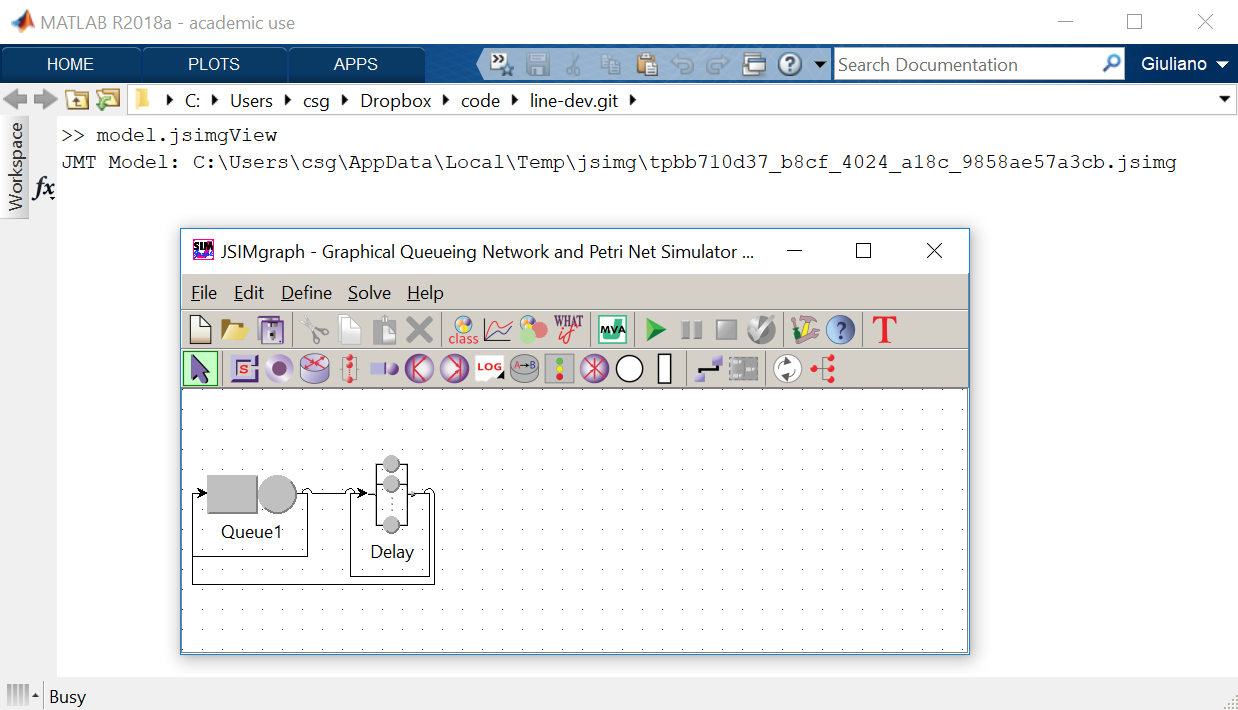
\includegraphics[width=14cm]{./images/jsimgView.png}
%  \caption{\texttt{Network.jsimgView} function}\label{FIG_jsimgView}
  \caption{jsimgView function}\label{jsimgView-function}
\end{figure}

Another way to debug a \textsc{Line} model is to transforming it into a MATLAB graph object, e.g.
\begin{lstlisting}
G = model.getGraph();
plot(G,'EdgeLabel',G.Edges.Weight,'Layout','Layered')
\end{lstlisting}
plots a graph of the network topology in term of stations only. In a similar manner, the following variant of the same command shows the model in terms of nodes, which corresponds to the internal representation within \textsc{Line}.
\begin{lstlisting}
[~,H] = model.getGraph();
plot(H,'EdgeLabel',H.Edges.Weight,'Layout','Layered')
\end{lstlisting}
The next figures shows the difference between the two commands for an open queueing network with two classes and class-switching. Weights on the edges correspond to routing probabilities. In the station topology on the left, note that since the \texttt{Sink} node is not a station, departures to the \texttt{Sink} are drawn as returns to the \texttt{Source}. The node topology on the right, illustrates all nodes, including certain \texttt{ClassSwitch} nodes that are automatically added by \textsc{Line} to apply the class-switching routing strategy. Double arcs between nodes indicate that both classes are routed to the destination.
\begin{figure}
  \centering
  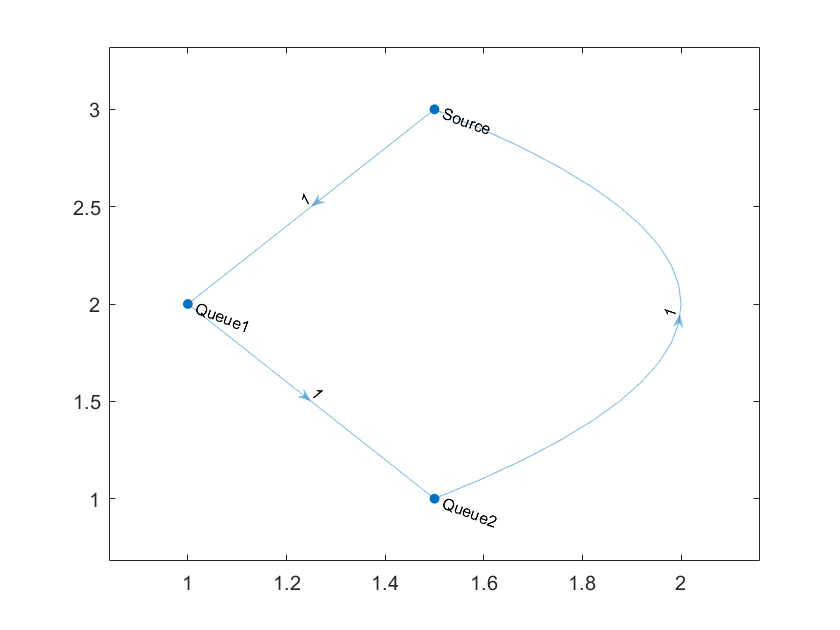
\includegraphics[width=7cm]{./images/getGraph_Stations.png}
  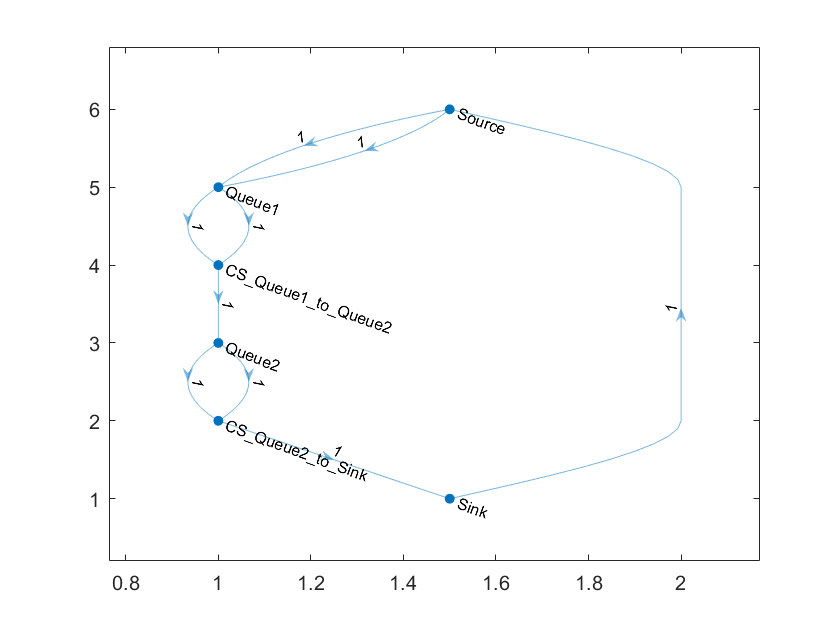
\includegraphics[width=7cm]{./images/getGraph_Nodes.png}
  \caption{\texttt{getGraph} function: station topology (left) and node topology (right) for a 2-class tandem queueing network with class-switching.}\label{FIG_getGraph}
\end{figure}

Furthermore, the graph properties concisely summarize the key features of the network
\begin{lstlisting}
>> G.Nodes
ans =
  2x5 table
      Name            Type           Sched    Jobs    ClosedClass1
    ________    _________________    _____    ____    ____________
    'Delay'     'Delay'       'inf'     5           1
    'Queue1'    'Queue'    'ps'      0           2
>> G.Edges
ans =
  3x4 table
          EndNodes          Weight    Rate        Class
    ____________________    ______    ____    ______________
    'Delay'     'Delay'      0.7        1     'ClosedClass1'
    'Delay'     'Queue1'     0.3        1     'ClosedClass1'
    'Queue1'    'Delay'        1      0.5     'ClosedClass1'
\end{lstlisting}
Here, \texttt{Edge.Weight} is the routing probability between the nodes, whereas \texttt{Edge.Rate} is the service rate of the source node.

\section{Model import and export}
%\section{Importing from BPMN}
%\section{Importing from JMT}
\textsc{Line} offers a number of scripts to import external models into \texttt{Network} object instances that can be analyzed through its solvers. %Similarly, a script is offered to convert a \texttt{Network} object instance into a MATLAB \texttt{.m} file for later re-use.
The available scripts are as follows:
\begin{itemize}
\item \texttt{JMT2LINE} imports a JMT simulation model (\texttt{.jsimg} or \texttt{.jsimw} file) instance.
\item \texttt{PMIF2LINE} imports a XML file containing a PMIF 1.0 model.
\end{itemize}
Both scripts require in input the filename and desired model name, and return a single output, e.g.,
\begin{lstlisting}
qn = PMIF2LINE([pwd,'\\examples\\data\\PMIF\\pmif_example_closed.xml'],'Mod1')
\end{lstlisting}
where \texttt{qn} is an instance of the \texttt{Network} class.

\texttt{Network} object can be saved in binary \texttt{.mat} files using MATLAB's standard \texttt{save} command. However, it is also possible to export a textual script that will dynamically recreate the same \texttt{Network} object. For example,
\begin{lstlisting}
example_closedModel_1; LINE2SCRIPT(model, 'script.m')
\end{lstlisting}
creates a new file \texttt{script.m} with code
\begin{lstlisting}
model = Network('model');
queue = Delay(model, 'Delay');
delay = Queue(model, 'Queue1', SchedStrategy.PS);
delay.setNumServers(1);
class1 = ClosedClass(model, 'ClosedClass1', 5, queue, 0);
queue.setService(class1, Cox2.fitMeanAndSCV(1.000000,1.000000));
delay.setService(class1, Cox2.fitMeanAndSCV(2.000000,1.000000));
P = cell(1);
P{1,1} = [0.7 0.3;1 0];
model.link(P);
\end{lstlisting}
that is equivalent to the model specified in \texttt{example\_closedModel\_1.m}.

\subsection{Creating a \textsc{Line} model using JMT}
Using the features presented in the previous section, one can create a model in JMT and automatically derive a corresponding \textsc{Line} script from it. For instance, the following command performs the import and translation into a script, e.g.,
\begin{lstlisting}
LINE2SCRIPT(JMT2LINE('myModel.jsimg'),'myModel.m')
\end{lstlisting}
transforms and save the given JSIMgraph model into a corresponding \textsc{Line} model.

\textsc{Line} also gives two static functions to inspect \texttt{jsimg} and \texttt{jsimw} files before conversion, i.e.,
\texttt{SolverJMT.jsimgOpen} and \texttt{SolverJMT.jsimwOpen} require as an input parameter only the JMT file name, e.g., 'myModel.jsimg'.



\chapter{Analysis methods}
\label{analysis-methods}

\section{Steady-state analysis}
\subsection{Station average performance}
\textsc{Line} decouples network specification from its solution, allowing to evaluate the same model with multiple solvers.
Model analysis is carried out in \textsc{Line} according to the following general steps:
\begin{description}
\item[Step 1: Definition of the model.] This proceeds as explained in the previous chapters.
\item[Step 2: Instantiation of the solver(s).] A solver is an instance of the \texttt{Solver} class. \textsc{Line} offers multiple solvers, which can be configured through a set of common and individual solver options. For example,
\begin{lstlisting}
solver = SolverJMT(model);
\end{lstlisting}
returns a handle to a simulation-based solver based on JMT, configured with default options.
\item[Step 3: Solution.] Finally, this step solves the network and retrieves the concrete values for the performance indexes of interest. This may be done as follows, e.g.,
\begin{lstlisting}
% QN(i,r): mean queue-length of class r at station i
QN = solver.getAvgQLen()
% UN(i,r): utilization of class r at station i
UN = solver.getAvgUtil()
% RN(i,r): mean response time of class r at station i (summed on visits)
RN = solver.getAvgRespT()
% TN(i,r): mean throughput of class r at station i
TN = solver.getAvgTput()
\end{lstlisting}
Alternatively, all the above metrics may be obtained in a single method call as
\begin{lstlisting}
[QN,UN,RN,TN] = solver.getAvg()
\end{lstlisting}
\end{description}
In the methods above, \textsc{Line} assigns station and class indexes (e.g., $i$, $r$) in order of creation in order of creation of the corresponding station and class objects. However, large models may be easier to debug by checking results using class and station names, as opposed to indexes. This can be done either by requesting \textsc{Line} to build a table with the result
\begin{lstlisting}
AvgTable = solver.getAvgTable()
\end{lstlisting}
which however tends to be a rather slow data structure to use in case of repeated invocations of the solver, or by indexing the matrices returned by \texttt{getAvg} using the model objects. That is, if the first instantiated node is \texttt{queue} with name \texttt{'MyQueue'} and the second instantiated class is \texttt{cclass} with name \texttt{'MyClass'}, then the following commands are equivalent
\begin{lstlisting}
QN(1,2)
QN(queue,cclass)
QN(model.getStationIndex('MyQueue'),model.getClassIndex('MyClass'))
\end{lstlisting}
Similar methods are defined to obtain aggregate performance metrics at chain level at each station, namely \texttt{getAvgQLenChain} for queue-lengths, \texttt{getAvgUtilChain} for utilizations, \texttt{getAvgRespTChain} for response times, \texttt{getAvgTputChain} for throughputs, and the \texttt{getAvgChain} method to obtain all the previous metrics.

\subsection{Station response time distribution}
\texttt{SolverFluid} supports the computation of response time distributions for individual classes through the \texttt{getCdfRespT} function. The function returns the response time distribution for every station and class. For example, the following code plots the cumulative distribution function at steady-state for class 1 jobs when they visit station 2:
\begin{lstlisting}
solver = SolverFluid(model);
FC = solver.getCdfRespT();
plot(FC{2,1}(:,2),FC{2,1}(:,1)); xlabel('t'); ylabel('Pr(RespT<t)');
\end{lstlisting}

\subsection{System average performance}
\textsc{Line} also allows users to analyze models for end-to-end performance indexes such a system throughput or system response time. However, in models with class switching the notion of system-wide metrics can be ambiguous. For example, consider a job that enters the network in one class and departs the network in another class. In this situation one may attribute system response time to either the arriving class or the departing one, or attempt to partition it proportionally to the time spent by the job within each class. In general, the right semantics depends on the aim of the study.

LINE tackles this issue by supporting only the computation of system performance indexes {\em by chain}, instead than by class. In this way, since a job switching from a class to another remains by definition in the same chain, there is no ambiguity in attributing the system metrics to the chain.  The solver functions \texttt{getAvgSys} and \texttt{getAvgSysTable} return system response time and system throughput per chain as observed: (i) upon arrival to the sink, for open classes; (ii) upon arrival to the reference station, for closed classes.

In some cases, it is possible that a chain visits multiple times the reference station before the job completes. This also affects the definition of the system averages, since in some applications one may want to avoid counting each visit as a completion of the visit to the system. In such cases, \textsc{Line} allows to specify which classes of the chain can complete at the reference station. For example, in the code below we require that a job visits reference station 1 twice, in classes 1 and 2, but completes at the reference station only when arriving in class 2. Therefore, the system response time will be counted between successive passages in class 2.
\begin{lstlisting}
class1 = ClosedClass(model, 'ClosedClass1', 1, queue, 0);
class2 = ClosedClass(model, 'ClosedClass2', 0, queue, 0);

class1.completes = false;

P = cell(2); % 2-classes model
P{1,1} = [0,1; 0,0]; % routing within class 1 (no switching)
P{1,2} = [0,0; 1,0]; % routing from class 1 into class 2
P{2,1} = [0,0; 1,0]; % routing within class 2 (no switching)
P{2,2} = [0,1; 0,0]; % routing from class 2 into class 2

model.link(P);
\end{lstlisting}
Note that \textsc{Line} does not allow a chain to complete at heterogeneous stations, therefore the \texttt{completes} property of a class always refers to the reference station for the chain.


\section{Specifying states}
In some analyses it is important to specify the state of the network, for example to assign the initial position of the jobs in a transient analysis. We thus discuss the native support in \textsc{Line} for state modeling.
\subsection{Station states}
We begin by explaining how to specify a state $s_0$. State modelling is supported only for stations with scheduling policies that depend on the number of jobs running or waiting at the node. For example, it is not supported for shortest job first (\texttt{SchedStrategy.SJF}) scheduling, in which state depends on the service time samples for the jobs.

Suppose that the network has $R$ classes and that service distributions are phase-type, i.e., that they inherit from \texttt{PhaseType}. Let $K_{r}$ be the number of phases for the service distribution in class $r$ at a given station. Then, we define three types of state variables:
\begin{itemize}
\item $c_j$: class of the job waiting in position $j\leq b$ of the buffer, out of the $b$ currently occupied positions. If $b=0$, then the state vector is indicated with a single empty element $c_1=0$.
\item $n_r$: total number of jobs of class $r$ in the station
\item $b_r$: total number of jobs of class $r$ in the station's buffer
\item $s_{rk}$: total number of jobs of class $r$ running in phase $k$ in the server
\end{itemize}
Here, by phase we mean the number of states of a distribution of class \texttt{PhaseType}. If the distribution is not Markovian, then there is a  single phase.
With these definitions, the table below illustrates how to specify in \textsc{Line} a valid state for a station depending on its scheduling strategy. All state variables are non-negative integers. The \texttt{SchedStrategy.EXT} policy is used for the \texttt{Source} node, which may be seen as a special station with an infinite pool of jobs sitting in the buffer and a dedicated server for each class $r=1,...,R$.
\begin{table}[thbp]
\renewcommand{\arraystretch}{1.2}
\centering
\caption{State descriptors for Markovian scheduling policies}
\begin{tabular}{|l|l|l|}
\hline
\textbf{Sched. strategy} & \textbf{Station state vector} & \textbf{State condition}\\
\hline
\texttt{EXT} & $[\texttt{Inf},s_{11},...,s_{1K_1},...,s_{R1},...,s_{RK_R}]$ & $\sum_k s_{rk}=1$, $\forall r$\\
\hline
\texttt{FCFS}, \texttt{HOL}, \texttt{LCFS} &   $[c_{b},...,c_{1},s_{11},...,s_{1K_1},...,s_{R1},...,s_{RK_R}]$& $\sum_{r}\sum_{k} s_{rk}=1$\\
\hline
\texttt{SEPT}, \texttt{RAND} &   $[b_{1},...,b_{R},s_{11},...,s_{1K_1},...,s_{R1},...,s_{RK_R}]$& $\sum_{r}\sum_{k} s_{rk}=1$\\
%\hline
%LEPT 	&NP	&			&$\checkmark$& 	&$\checkmark$	&&$\checkmark$&	\\
%\hline
%LJF & \\
\hline
\texttt{PS}, \texttt{DPS}, \texttt{GPS}, \texttt{INF}	&   $[s_{11},...,s_{1K_1},...,s_{R1},...,s_{RK_R}]$& None\\
%\hline
%SJF & Not supported.\\
\hline
\end{tabular}
\label{TAB_state_policies}
\end{table}

States can be manually specified or enumerated automatically. \textsc{Line} library functions for handling and generating states are as follows:
\begin{itemize}
\item \texttt{State.fromMarginal}: enumerates all states that have the same marginal state $[n_{1},n_{2},...,n_{R}]$.
\item \texttt{State.fromMarginalAndRunning}: restricts the output of \texttt{State.fromMarginal} to states with given number of running jobs, irrespectively of the service phase in which they currently run.
\item \texttt{State.fromMarginalAndStarted}: restricts the output of \texttt{State.fromMarginal} to states with given number of running jobs, all assumed to be in service phase $k=1$.
\item \texttt{State.fromMarginalBounds}: similar to \texttt{State.fromMarginal}, but produces valid states between given minimum and maximum of resident jobs.
\item \texttt{State.toMarginal}: extracts statistics from a state, such as the total number of jobs in a given class that are running at the station in a certain phase.
\end{itemize}
Note that if a function call returns an empty state (\texttt{[]}), this should be interpreted as an indication that no valid state exists that meets the required criteria. Often, this is because the state supplied in input is invalid.

\subsubsection{Example} We consider the example network in \texttt{example\_closedModel\_4.m}. We look at the state of station 3, which is a multi-server FCFS station. There are 4 classes all having exponential service times except class 2 that has Erlang-2 service times. We are interested to states with 2 running jobs in class 1 and 1 in class 2, and with 2 jobs, respectively of classes 3 and 4, waiting in the buffer. We can automatically generate this state space, which we store in the \texttt{space} variable, as:
\begin{lstlisting}
>> example_closedModel_4;
>> space = State.fromMarginalAndRunning(model,3,[2,1,1,1],[2,1,0,0])
space =
     4     3     2     1     0     0     0
     4     3     2     0     1     0     0
     3     4     2     1     0     0     0
     3     4     2     0     1     0     0
\end{lstlisting}
Here, each row of \texttt{space} corresponds to a valid state. The argument \texttt{[2,1,1,1]} gives the number of jobs in the node for the 4 classes, while \texttt{[2,1,0,0]} gives the number of running jobs in each class. This station has four valid states, differing on whether the class-2 job runs in the first or in the second phase of the Erlang-2 and on the relative position of the jobs of class 3 and 4 in the waiting buffer.

To obtain states where the jobs have just started running, we can instead use
\begin{lstlisting}
>> space = State.fromMarginalAndStarted(model,3,[2,1,1,1],[2,1,0,0])
space =
     4     3     2     1     0     0     0
     3     4     2     1     0     0     0
\end{lstlisting}
If we instead remove the specification of the running jobs, we can use \texttt{State.fromMarginal} to generate all possible combinations of states depending on the class and phase of the running jobs. In the example, this returns a space of 20 possible states.
\begin{lstlisting}
>> space = State.fromMarginal(model,3,[2,1,1,1],[2,1,0,0])
space =
     4     3     2     1     0     0     0
     4     3     2     0     1     0     0
     4     2     2     0     0     1     0
     4     1     1     1     0     1     0
     4     1     1     0     1     1     0
     3     4     2     1     0     0     0
     3     4     2     0     1     0     0
     3     2     2     0     0     0     1
     3     1     1     1     0     0     1
     3     1     1     0     1     0     1
     2     4     2     0     0     1     0
     2     3     2     0     0     0     1
     2     1     1     0     0     1     1
     1     4     1     1     0     1     0
     1     4     1     0     1     1     0
     1     3     1     1     0     0     1
     1     3     1     0     1     0     1
     1     2     1     0     0     1     1
     1     1     0     1     0     1     1
     1     1     0     0     1     1     1
\end{lstlisting}
\subsubsection{Assigning a state to a station}
Given a single or multiple states, it is possible to assign the initial state to a station using the \texttt{setState} function on that station's object. To cope with multiple states, \textsc{Line} offers the possibility to specify a prior probability on the initial states, so that if multiple states have a non-zero prior, then the solver will need to analyze the network from all those states and weight the results according to the prior probabilities. The default prior value assigned probability 1.0 to the {\em first} specified state. The functions \texttt{setStatePrior} and \texttt{getStatePrior} of the \texttt{Station} class can be used to check and change the prior probabilities for the supplied initial states.

\subsection{Network states}
A collection of states that are valid for each station is not necessarily valid for the network as a whole. For example, if the sum of jobs of a closed class exceeds the population of the class, then the network state would be invalid. To identify these situations, \textsc{Line} requires to specify the initial state of a network using functions supplied by the \texttt{Network} class. These functions are \texttt{initFromMarginal}, \texttt{initFromMarginalAndRunning}, and \texttt{initFromMarginalAndStarted}. They require a matrix with elements \texttt{n}$(i,r)$ specifying the total number of resident class-$r$ jobs at node $i$ and the latter two require a matrix \texttt{s}$(i,r)$ with the number of running (or started) class-$r$ jobs at node $i$. The user can also manually verify if the supplied network state is going to be valid using \texttt{State.IsValid}.

It is also possible to request \textsc{Line} to automatically identify a valid initial state, which is done using the \texttt{initDefault} function available in the \texttt{Network} class. This is going to select a state where:
\begin{itemize}
\item no jobs in open classes are present in the network;
\item jobs in closed classes all start at their reference stations;
\item the server of reference stations are occupied in order of class id, i.e., jobs in the firstly created class are assigned to the server in phase 1, then spare servers are allocated to the second class in phase 1, and so forth;
\item if the scheduling strategy requires it, jobs are ordered in the buffer by class, with the firstly created class at the head and the lastly created class at the tail of the buffer.
\end{itemize}

Lastly, the \texttt{initFromAvgQLen} is a wrapper for \texttt{initFromMarginal} to initialize the system as close as possible to the average steady-state distribution of the network. Since averages are typically not integer-valued, this function rounds the average values to the nearest integer and adjusts the result to ensure feasibility of the initialization.

\subsection{Initialization of transient classes}
Because of class-switching, it is possible that a class $r$ with a non-empty population at time $t=0$ becomes empty at some position time $t'>t$ without ever being visited again by any job. \texttt{LINE} allows one to place jobs in transient classes and therefore it will not trigger an error in the presence of this situation. If a user wishes to prohibit the use of a class at a station, it is sufficient to specify that the corresponding service process uses the \texttt{Disabled} distribution.

Certain solvers may incur problems in identifying that a class is transient and in setting to zero its steady-state measures. For example, the \texttt{JMT} solver uses an heuristic whereby a class is considered transient if it has fewer events than jobs initially placed in the corresponding chain the class belongs to. For such classes, \texttt{JMT} will set the values of steady-state performance indexes to zero.


\section{Transient analysis}
So far, we have seen how to compute steady-state average performance indexes, which are given by
\[
E[n]=\lim\limits_{t\to +\infty }E[n(t)]
\]
where $n(t)$ is an arbitrary performance index, e.g., the queue-length of a given class at time $t$.

We now consider instead the computation of the quantity $E[n(t)|s_0]$, which is the {\em transient average} of the performance index, conditional on a given initial system state $s_0$. Compared to $n(t)$, this quantity averages the system state at time $t$ across all possible evolutions of the system from state $s_0$ during the $t$ time units, weighted by their probability. In other words, we observe all possible stochastic evolutions of the system from state $s_0$ for $t$ time units, recording the final values of $n(t)$ in each trajectory, and finally average the recorded values at time $t$ to obtain $E[n(t)|s_0]$.

\subsection{Computing transient averages}
At present, \textsc{Line} supports only transient computation of queue-lengths, throughputs and utilizations using the \texttt{CTMC} and \texttt{FLUID} solvers. Transient response times are not currently supported, as they do not always obey Little's law.

The computation of transient metrics proceeds similarly to the steady-state case. We first obtain the handles for transient averages:
\begin{lstlisting}
[Qt,Ut,Tt] = model.getTransientHandlers();
\end{lstlisting}
After solving the model, we will be able to retrieve {\em both} steady-state and transient averages as follows
\begin{lstlisting}
[QNt,UNt,TNt] = solver{s}.getTransientAvg(Qt,Ut,Tt)
plot(QNt{1,1}(:,2), QNt{1,1}(:,1))
\end{lstlisting}
The transient average queue-length at node $i$ for class $r$ is stored within \texttt{QNt\{i,r\}}.%, which is a MATLAB \texttt{timeseries} object. This object class can be plotted directly. Data and time values in the time series can also be accessed using the \texttt{Data} and \texttt{Time} fields within the object.

Note that the above code does not show how to specify a maximum time $t$ for the output time series. This can be done using the \texttt{timespan} field of the options, as described later in the solvers chapter. %The solver will automatically solve the network until a large enough $t$ is reached so that the network is approximately in steady-state. This is done to ensure that average steady-state performance metrics can also be determined as an output of the transient solution.

\subsection{First passage times into stations}
When the model is in a transient, the average state seen upon arrival to a station changes over time. That is, in a transient, successive visits by a job may experience different response time distributions. The function \texttt{getTransientCdfRespT}, implemented by \texttt{SolverJMT} offers the possibility to obtain this distribution given the initial state specified for the model. As time passes, this distribution will converge to the steady-state one computed by solvers equipped with the function \texttt{getCdfRespT}.

However, in some cases one prefers to replace the notion of response time distribution in transient by the one of \emph{first passage time}, i.e., the distribution of the time to complete the {\em first visit} to the station under consideration. The function \texttt{getTransientCdfFirstPassT} provides this distribution, assuming as initial state the one specified for the model, e.g., using \texttt{setState} or \texttt{initDefault}. This function is available only in \texttt{SolverFluid} and has a similar syntax as \texttt{getCdfRespT}.

\section{Sensitivity analysis and numerical optimization}
\label{sensitivity-analysis-and-numerical-optimization}
Frequently, performance and reliability analysis requires to change one or more model parameters to see the sensitivity of the results or to optimize some goal function. In order to do this efficiently, we discuss the internal representation of the \texttt{Network} objects used within the \textsc{Line} solvers. By applying changes directly to this internal representation it is possible to considerably speed-up the sequential evaluation of several models.

\subsection{Internal representation of the model structure}
For efficiency reasons, once a user requests to solve a \texttt{Network}, \textsc{Line} calls internally generates a static representation of the network structure using the \texttt{refreshStruct} function. This function returns a representation object that is then passed on to the chosen solver to parameterize the analysis.

The representation used within \textsc{Line} is the \texttt{NetworkStruct} class, which describes an extended multiclass queueing network with class-switching and Coxian service times. The representation can be obtained as follows
\begin{lstlisting}
qn = model.getStruct()
\end{lstlisting}
The table below presents the properties of the \texttt{NetworkStruct} class.

\begin{table}[thbp]
{\footnotesize
\renewcommand{\arraystretch}{1.2}
\centering
\caption{\texttt{NetworkStruct} properties} %{Legend: $i,j=$ stations; $r,s=$ classes; $c=$ chain; $k=$ phase; $t=$ state}}
\begin{tabular}{|l|l|p{9.5cm}|}
\hline
\textbf{Field} & \textbf{Type} & \textbf{Description} \\
\hline
\texttt{cap}$(i)$ & \texttt{integer} & Total capacity at station $i$ \\\hline
\texttt{chains}$(c,r)$ & \texttt{logical} &  \texttt{true} if class $r$ is in chain $c$, or \texttt{false} otherwise \\\hline
\texttt{classcap}$(i,r)$ & \texttt{integer} & Maximum buffer capacity available to class $r$ at station $i$ \\\hline
\texttt{classname}$\{r\}$ & \texttt{string} & Name of class $r$\\\hline
\texttt{classprio}$(r)$ & \texttt{integer} & Priority of class $r$ (0 = highest priority)\\\hline
\texttt{csmask}$(r,s)$ & \texttt{logical} & true if class $r$ can switch into class $s$ at some node\\\hline
{\texttt{isstation}}$(i)$ & {\texttt{logical}} & true if node $i$ is a station\\\hline
{\texttt{isstateful}}$(i)$ & {\texttt{logical}} & true if node $i$ is a stateful node\\\hline
\texttt{mu}$\{i,r\}(k)$ & \texttt{double} & Coxian service or arrival rate in phase $k$ for class $r$ at station $i$, with \texttt{mu}$\{i,r\}=$\texttt{NaN} if \texttt{Disabled} and \texttt{mu}$\{i,r\}=10^7$ if \texttt{Immediate}.\\\hline
\texttt{nchains} & \texttt{integer} & Number of chains in the network\\\hline
%\texttt{nchainjobs}$(c)$ & \texttt{integer} & Number of jobs in chain $c$\\\hline
\texttt{nclasses} & \texttt{integer} & Number of classes in the network\\\hline
\texttt{nclosedjobs} & \texttt{integer} & Total number of jobs in closed classes\\\hline
\texttt{njobs}$(r)$ & \texttt{integer} & Number of jobs in class $r$ (\texttt{Inf} for open classes)\\\hline
\texttt{nnodes} & \texttt{integer} & Number of nodes in the network\\\hline
\texttt{nservers}$(i)$ & \texttt{integer} & Number of servers at station $i$\\\hline
\texttt{nstations} & \texttt{integer} & Number of stations in the network\\\hline
\texttt{nstateful} & \texttt{integer} & Number of stateful nodes in the network\\\hline
\texttt{nodenames}$\{i\}$ & \texttt{string} & Name of node $i$\\\hline
\texttt{nodetypes}$\{i\}$ & \texttt{string} & Type of node $i$ (e.g., \texttt{NodeType.Sink})\\\hline
\texttt{nvars} & \texttt{integer} & Number of local state variables at stateful nodes\\\hline
\texttt{phases}$(i,r)$ & \texttt{integer} & Number of phases for service process of class $r$ at station $i$\\\hline
\texttt{phi}$\{i,r\}(k)$ & \texttt{double} & Coxian completion probability in phase $k$ for class $r$ at station $i$\\\hline
\texttt{rates}$(i,r)$ & \texttt{double} & Service rate of class $r$ at station $i$ (or  arrival rate if $i$ is a \texttt{Source})\\\hline
\texttt{refstat}$(r)$ & \texttt{integer} & Index of reference station for class $r$ \\\hline
\texttt{rt}$(idx_{ir},idx_{js})$  & \texttt{double} & Probability of routing from stateful node $i$ to $j$, switching class from $r$ to $s$ where, e.g., $idx_{ir}=(i-1)*\texttt{nclasses}+r$.\\\hline
\texttt{rtnodes}$(idx_{ir},idx_{js})$  & \texttt{double} & Same as \texttt{rt}, but $i$ and $j$ are nodes, not necessarily stateful ones.\\\hline
\texttt{rtfun}$(\texttt{st1},\texttt{st2})$  & \texttt{matrix} & State-dependent routing table given initial (\texttt{st1}) and final (\texttt{st2}) state cell arrays. Table entries defined as in \texttt{rt}.\\\hline
\texttt{schedparam}$(i,r)$ & \texttt{double} &  Parameter for class $r$ strategy at station $i$\\\hline
\texttt{sched}$\{i\}$& \texttt{cell} & Scheduling strategy at station $i$ (e.g., \texttt{SchedStrategy.PS})\\\hline
\texttt{schedid}$(i)$ & \texttt{integer} & Scheduling strategy id at station $i$ (e.g., \texttt{SchedStrategy.ID\_PS})\\\hline
\texttt{sync}$\{s\}$ & \texttt{struct} & Data structure specifying a synchronization $s$ among nodes\\\hline
\texttt{scv}$(i,r)$ & \texttt{double} & Squared coefficient of variation of class $r$ service times at station $i$ (or inter-arrival times if station $i$ is a \texttt{Source})\\\hline
\texttt{space}$\{t\}$  & \texttt{integer} & The $t$-th state in the state space (or a portion thereof). This field may be initially empty and updated by the solver during execution.\\\hline
\texttt{state}$\{i\}$ & \texttt{integer} & Current state of stateful node $i$. This field may be initially empty and updated by the solver during execution.\\\hline
\texttt{visits}$\{c\}(i,r)$  & \texttt{double} & Number of visits that a job in chain $c$ pays to node $i$ in class $r$\\\hline
\texttt{varsparam}$\{i\}$  & \texttt{double} & Parameters for local variable instantiation at stateful node $i$\\
\hline
\end{tabular}
}
\label{TAB_QN}
\end{table}
\subsection{Fast parameter update}
Successive invocations of \texttt{getStruct()} will return a cached copy of the \texttt{NetworkStruct} representation, unless the user has called \texttt{model.refreshStruct()} or \texttt{model.reset()} in-between the invocations. The \texttt{refreshStruct} function regenerates the internal representation, while \texttt{reset} destroys it, together with all other representations and cached results stored in the \texttt{Network} object. In the case of \texttt{reset}, the internal data structure will be regenerated at the next \texttt{refreshStruct()} or \texttt{getStruct()} call.

The performance cost of updating the representation can be significant, as some of the structure array field require a dedicated algorithm to compute. For example, finding the chains in the model requires an analysis of the weakly connected components of the network routing matrix. For this reason, the \texttt{Network} class provides several functions to selectively refresh only part of the \texttt{NetworkStruct} representation, once the modification has been applied to the objects (e.g., stations, classes, ...) used to define the network. These functions are as follows:
\begin{itemize}
\item \texttt{refreshArrival}: this function should be called after updating the inter-arrival distribution at a \texttt{Source}. %    The function is identical to \texttt{refreshService}.
\item \texttt{refreshCapacity}: this function should be called after changing buffer capacities, as it updates the \texttt{capacity} and \texttt{classcapacity} fields.
\item \texttt{refreshChains}: this function should be used after changing the routing topology, as it refreshes the \texttt{rt}, \texttt{chains}, \texttt{nchains}, \texttt{nchainjobs}, and \texttt{visits} fields.
\item \texttt{refreshPriorities}: this function updates class priorities in the \texttt{classprio} field.
%\item \texttt{refreshRates}: this function should be called after changing a service time distribution at a station as it updates the \texttt{rates} and \texttt{scv} fields.
%\item \texttt{refreshRoutingMatrix}: updates the \texttt{rt} field.
\item \texttt{refreshScheduling}: updates the \texttt{sched}, \texttt{schedid}, and \texttt{schedparam} fields.
\item \texttt{refreshService}: updates the \texttt{mu}, \texttt{phi}, \texttt{phases}, \texttt{rates} and \texttt{scv} fields.
\end{itemize}
For example, suppose we wish to update the service time distribution for class-1 at node 1 to be exponential with unit rate. This can be done efficiently as follows:
\begin{lstlisting}
queue.setService(class1, Exp(1.0));
model.refreshService;
\end{lstlisting}

\subsection{Refreshing a network topology with non-probabilistic routing}
The \texttt{resetNetwork} function should be used before changing a network topology with non-probabilistic routing. It will destroy by default all class switching nodes. This can be avoided if the function is called as, e.g., \texttt{model.resetNetwork(false)}. The default behavior is though shown in the next example
\begin{lstlisting}
>> model = Network('model');
node{1} = ClassSwitch(model,'CSNode',[0,1;0,1]);
node{2} = Queue(model, 'Queue1', SchedStrategy.FCFS);
>> model.getNodes
ans =
  2x1 cell array
    {1x1 ClassSwitch}
    {1x1 Queue}
>> model.resetNetwork
ans =
  1x1 cell array
    {1x1 Queue}
\end{lstlisting}
As shown, \texttt{resetNetwork} updates the station indexes and the revised list of nodes that compose the topology is obtained as a return parameter. To avoid stations to change index, one may simply create  \texttt{ClassSwitch} nodes as last before solving the model. This node list can be employed as usual to reinstantiate new stations or \texttt{ClassSwitch} nodes. The \texttt{addLink}, \texttt{setRouting}, and possibly the \texttt{setProbRouting} functions will also need to be re-applied as described in the previous sections.

\subsection{Saving a network object before a change}
The \texttt{Network} object, and its inner objects that describe the network elements, are always passed by reference. The \texttt{copy} function should be used to clone \textsc{Line} objects, for example before modifying a parameter for a sensitivity analysis. This function recursively clones all objects in the model, therefore creating an independent copy of the network. For example, consider the following code
\begin{lstlisting}
modelByRef = model; modelByRef.setName('myModel1');
modelByCopy = model.copy; modelByCopy.setName('myModel2');
\end{lstlisting}
Using the \texttt{getName} function it is then possible to verify that \texttt{model} has now name \texttt{'myModel1'}, since the first assignment was by reference. Conversely, \texttt{modelByCopy.setName} did not affect the original \texttt{model} since this is a clone of the original network.



\chapter{Network solvers}
\label{Network-solvers}
\section{Overview}
Solvers analyze objects of class \texttt{Network} to return average, transient, distributions, or state probability metrics. A solver can implement one or more {\em methods}, which although sharing a similar overall solution strategy, they can differ significantly from each other in the way this is actually implemented and on wether the final solution is exact or approximate.

The \texttt{method} field in the options structure array passed to a solver can be used to select the desired method, e.g., \texttt{options.method='default'} requires the solver to use default options, while \texttt{options.method='exact'} requires to solve the model exactly, if an exact solution method is available.

In what follows, we describe the general characteristics and supported model features for each solver available in \textsc{LINE} and their methods.
%By definition, a solver cannot modify the \texttt{Network} object.
\subsubsection{Available solvers}
\noindent The following \texttt{Network} solvers are available within \textsc{Line} 2.0.0-ALPHA:
%\section{Solvers}
%\label{SEC_solvers}
%\begin{table}[t!]
%\renewcommand{\arraystretch}{1.2}
%\centering
%\begin{tabular}{|l|c|c|c|c|c|c|}
%\cline{2-6}
%\multicolumn{1}{c|}{}&\multicolumn{5}{c|}{\textbf{Solver}}\\
%\cline{1-6}
%\textbf{Feature}&\texttt{MVA}	&\texttt{CTMC}&\texttt{FLUID}	 	&\texttt{JMT} 	&\texttt{SSA}\\
%\hline
%%CQN &  $\checkmark$  & $\checkmark$  & $\checkmark$  & $\checkmark$& $\checkmark$ \\
%Cox & $\checkmark$  & $\checkmark$  & $\checkmark$  & $\checkmark$& $\checkmark$ \\
%CS & $\checkmark$  & $\checkmark$ & $\checkmark$ &$\checkmark$ & $\checkmark$\\
%RE &  &  & API-only & & \\
%%TD &  &  &  & & $\checkmark$\\
%\hline
%\end{tabular}
%\caption{Advanced model features supported by the \textsc{Line} solvers}
%\label{TAB_solver_features}
%\end{table}
%Table~\ref{TAB_solver_features} summarizes the solvers included in \textsc{Line} and the model features they support. As indicated in Table~\ref{TAB_solver_features}, the RE feature is currently supported only via the LINE API. Conversely, the AVG indexes are available both in the \textsc{Line} modeling language and in the API. A detailed description of the solvers is as follows:
\begin{itemize}
\item \texttt{AUTO}: This solver uses an algorithm to select the best solution method for the model under consideration, among those offered by the other solvers. Analytical solvers are always preferred to simulation-based solvers. This solver is implemented by the \texttt{SolverAuto} class.
\item \texttt{CTMC}: This is a solver that returns the exact values of the performance metrics by explicit generation of the continuous-time Markov chain (CTMC) underpinning the model. As the CTMC typically incurs state-space explosion, this solver can successfully analyze only small models. The {CTMC} solver is the only method offered within \textsc{Line} that can return an exact solution on all Markovian models, all other solvers are either approximate or are simulators. This solver is implemented by the \texttt{SolverCTMC} class.
\item \texttt{FLUID}: This solver analyzes the model by means of an approximate fluid model, leveraging a representation of the queueing network as a system of ordinary differential equations (ODEs). The fluid model is approximate, but if the servers are all PS or INF, it can be shown to become exact in the limit where the number of users and the number of servers in each node grow to infinity~\cite{pere.casa13}. This solver is implemented by the \texttt{SolverFluid} class.
\item \texttt{JMT}: This is a solver that uses a model-to-model transformation to export the \textsc{Line} representation into a JMT simulation model~\cite{BerCS07}. This solver can analyze also non-Markovian models, in particular those involving deterministic or Pareto distributions, or empirical traces. This solver is implemented by the \texttt{SolverJMT} class.
\item \texttt{MAM}: This is a matrix-analytic method solver, which relies on quasi-birth death (QBD) processes to analyze open queueing systems. This solver is implemented by the \texttt{SolverMAM} class.
\item \texttt{MVA}: This is a solver based on approximate and exact mean-value analysis. This solver is typically the fastest and offers very good accuracy in a number of situations, in particular models where stations have a single-server. This solver is implemented by the \texttt{SolverMVA} class. %The {MVA} solver in \textsc{Line} allow for queue-dependent (QD) stations, where the rate of processing depends on the queue-length, such as nodes with multiple servers. However, {MVA} cannot produce response time distributions, due to an intrinsic limitation of the solution paradigm. A detailed description of the {MVA} algorithm used in \textsc{Line} 2.0.0-ALPHA is provided in \cite{casale2015qdamva}.
\item \texttt{NC}: This solver uses a combination of methods based on the normalizing constant of state probability to solve a model. The underpinning algorithm are particularly useful to compute marginal and joint state probabilities in queueing network models. This solver is implemented by the \texttt{SolverNC} class.
\item \texttt{SSA}: This is a discrete-event simulator based on the CTMC representation of the model. The solver is implemented in MATLAB language and thus tends to offer lower speed than JMT, but the model execution can be easily parallelized using MATLAB's {\em spmd} construct. This solver is implemented by the \texttt{SolverSSA} class.
\end{itemize}

%\subsubsection{{Layered network} solvers}
%\noindent In addition, the following \texttt{LayeredNetwork} solvers are available:
%\begin{itemize}
%\item \texttt{LQNS}: This is a wrapper of the LQNS solver. It assumes that both \texttt{lqns} and \texttt{lqsim} are available on the operating system path so that they can be found by MATLAB's \texttt{system} API.
%\item \texttt{LN}: This is \textsc{Line}'s own layered network solver. Compared to the published version, the current release is based on a SRVN-style decomposition, whereby each server is modelled using a separate submodel.
%\end{itemize}

\section{Solution algorithms}
\subsection{\texttt{AUTO}}
The \texttt{SolverAuto} class provides interfaces to the core solution functions (e.g., \texttt{getAvg}, ...) that dynamically bind to one of the other solvers implemented in \textsc{Line} (\texttt{CTMC}, \texttt{NC}, ...). It is often not possible to identify the best solver without some performance results on the model, for example to determine if it operates in light, moderate, or heavy-load regime.

Therefore, heuristics are used to identify a solver based on structural properties of the model, such as based on the scheduling strategies used at the stations as well as the number of jobs, chains, and classes. Such heuristics, though, are independent of the core function called, thus it is possible that the optimal solver does not  support the specific function called (e.g., \texttt{getTranAvg}). In such cases \texttt{SolverAuto} determines what other solvers would be feasible and prioritizes them in execution time order, with the fastest one on average having the higher priority. Eventually, the solver will be always able to identify a solution strategy, through at least simulation-based solvers such as \texttt{JMT} or \texttt{SSA}.

\subsection{\texttt{CTMC}}
The \texttt{SolverCTMC} class solves the model by first generating the infinitesimal generator of the \texttt{Network} and then calling an appropriate solver. Steady-state analysis is carried out by solving the global balance equations defined by the infinitesimal generator. If the \texttt{keep} option is set to true, the solver will save the infinitesimal generator in a temporary file and its location will be shown to the user.

Transient analysis is carried out by numerically solving Kolmogorov's forward equations using MATLAB's ODE solvers. The range of integration is controlled by the \texttt{timespan} option. The ODE solver choice is the same as for \texttt{SolverFluid}.

The CTMC solver heuristically limits the solution to models with no more than 6000 states. The \texttt{force} option needs to be set to true to bypass this control. In models with infinite states, such as networks with open classes, the \texttt{cutoff} option should be used to reduce the CTMC to a finite process. If specified as a scalar value, \texttt{cutoff} is the maximum number of jobs that a class can place at an arbitrary station. More generally, a matrix assignment of \texttt{cutoff} indicates to \texttt{LINE} that \texttt{cutoff}$(i,r)$ is the maximum number of jobs of class $r$ that can be placed at station $i$.

%{
%\begin{table}[thbp]
%\footnotesize
%\renewcommand{\arraystretch}{1.2}
%\centering
%\caption{SolverCTMC methods}
%\begin{tabular}{|l|l|}
%\hline
%\textbf{Method} & \textbf{Description}\\
%\hline
%\texttt{std} &  \\
%\texttt{exact} &  \\
%\hline
%\end{tabular}
%\label{TAB_CTMC_methods}
%\end{table}
%}

\subsection{\texttt{FLUID}}
This solver is based on the system of fluid ordinary differential equations for INF-PS queueing networks presented in \cite{PerC17}.

The fluid ODEs are normally solved with the \texttt{'NonNegative'} ODE solver option enabled. Four types of ODE solvers are used: \emph{fast} or \emph{accurate}, the former only if \texttt{options.iter\_tol}$> 10^{-3}$, and \emph{stiff} or \emph{non-stiff}, depending on the value of \texttt{options.stiff}. The default choice of solver is stored in the following static functions:
\begin{itemize}
\item \texttt{Solver.accurateStiffOdeSolver}, set to MATLAB's \texttt{ode15s}.
\item \texttt{Solver.accurateOdeSolver}, set to \texttt{ode45}.
\item \texttt{Solver.fastStiffOdeSolver}, set to \texttt{ode23s}.
\item \texttt{Solver.fastOdeSolver}, set to \texttt{ode23}.
\end{itemize}

ODE variables corresponding to an infinite number of jobs, as in the job pool of a source station, or to jobs in a disabled class are not included in the solution vector. These rules apply also to the \texttt{options.init\_sol} vector.

The solution of models with FCFS stations maps these stations into corresponding PS stations where the service rates across classes are set identical to each other with a service distribution given by a mixture of the service processes of the service classes. The mixture weights are determined iteratively by solving a sequence of PS models until convergence. Upon initializing FCFS queues, jobs in the buffer are all initialized in the first phase of the service.

%{
%\begin{table}[thbp]
%\footnotesize
%\renewcommand{\arraystretch}{1.2}
%\centering
%\caption{SolverFluid methods}
%\begin{tabular}{|l|l|}
%\hline
%\textbf{Method} & \textbf{Description}\\
%\hline
%\texttt{std} &  \\
%\texttt{exact} &  \\
%\hline
%\end{tabular}
%\label{TAB_Fluid_methods}
%\end{table}
%}

\subsection{\texttt{JMT}}
The class is a wrapper for the \texttt{JMT} simulation and consists of a model-to-model transformation from the \texttt{Network} data structure into the JMT's input XML format (\texttt{.jsimg}) and a corresponding parser for JMT's results. In the transformation, artificial nodes will be automatically added to the routing table to represent class-switching nodes used in the simulator to specify the switching rules. One such class-switching node is defined for every ordered pair of stations $(i,j)$ such that jobs change class in transit from $i$ to $j$.

Upon invocation, the \texttt{JMT} JAR archive will be searched in the MATLAB path and if unavailable automatically downloaded.
%\texttt{JMT} allows to specify the initial number of jobs in a queue, but their ordering within the buffer and the selection of the ones running is internally randomized.

%{
%\begin{table}[thbp]
%\footnotesize
%\renewcommand{\arraystretch}{1.2}
%\centering
%\caption{SolverJMT methods}
%\begin{tabular}{|l|l|}
%\hline
%\textbf{Method} & \textbf{Description}\\
%\hline
%\texttt{std} &  \\
%\texttt{exact} &  \\
%\hline
%\end{tabular}
%\label{TAB_JMT_methods}
%\end{table}
%}
\subsection{\texttt{MAM}}
This is a basic solver for some Markovian open queueing systems that can be analyzed using matrix analytic methods. The solver at the moment is a basic wrapper for the {BU tools} library for matrix-analytic methods~\cite{Hor17}. At present, it is not possible to solve a queueing network model using \texttt{SolverMAM}.

%{
%\begin{table}[thbp]
%\footnotesize
%\renewcommand{\arraystretch}{1.2}
%\centering
%\caption{SolverMAM methods}
%\begin{tabular}{|l|l|}
%\hline
%\textbf{Method} & \textbf{Description}\\
%\hline
%\texttt{std} &  \\
%\texttt{exact} &  \\
%\hline
%\end{tabular}
%\label{TAB_MAM_methods}
%\end{table}
%}

\subsection{\texttt{MVA}}
The solver is primarily based on the Bard-Schweitzer approximate mean value analysis (AMVA) algorithm (\texttt{options.method='default'}), but also offers and implementation of the exact MVA algorithm (\texttt{options.method='exact'}). Non-exponential service times in FCFS nodes are treated using a M/G/1-type approximation. Multi-server FCFS is dealt with using a slight modification of the Rolia-Sevcik method~\cite{roli.sevc95}. DPS queues are analyzed with a time-scale separation method, so that for an incoming job of class $r$ and weight $w_r$, classes with weight $w_s\geq 5w_r$ are replaced by high-priority classes that are analyzed using the standard MVA priority approximation. Conversely the remaining classes are treated by weighting the queue-length seen upon arrival in class $s\neq r$ by the correction factor $w_s/w_r$.
%{
%\begin{table}[thbp]
%\footnotesize
%\renewcommand{\arraystretch}{1.2}
%\centering
%\caption{SolverMVA methods}
%\begin{tabular}{|l|l|}
%\hline
%\textbf{Method} & \textbf{Description}\\
%\hline
%\texttt{std} &  \\
%\texttt{exact} &  \\
%\hline
%\end{tabular}
%\label{TAB_MVA_methods}
%\end{table}
%}

\subsection{\texttt{NC}}
The \texttt{SolverNC} class implements a family of solution algorithms based on the normalizing constant of state probability of product-form queueing networks. Contrary to the other solvers, this method typicallly maps the problem to certain multidimensional integrals, allowing the use of numerical methods such as MonteCarlo sampling and asymptotic expansions in their approximation.
%{
%\begin{table}[thbp]
%\footnotesize
%\renewcommand{\arraystretch}{1.2}
%\centering
%\caption{SolverNC methods}
%\begin{tabular}{|l|l|}
%\hline
%\textbf{Method} & \textbf{Description}\\
%\hline
%\texttt{std} &  \\
%\texttt{exact} &  \\
%\hline
%\end{tabular}
%\label{TAB_NC_methods}
%\end{table}
%}

\subsection{\texttt{SSA}}
The \texttt{SolverSSA} class is a basic stochastic simulator for continuous-time Markov chains. It reuses some of the methods that underpin \texttt{SolverCTMC} to generate the network state space and subsequently simulates the state dynamics by probabilistically choosing one among the possible events that can incur in the system, according to the state spaces of each of node in the network. For efficiency reasons, states are tracked at the level of individual stations, and hashed. The state space is not generated upfront, but rather stored during the simulation, starting from the initial state. If the initialization of a station generates multiple possible initial states, \texttt{SSA} initializes the model using the first state found. The list of initial states for each station can be obtained using the \texttt{getInitState} functions of the \texttt{Network} class.

The \texttt{SSA} solver offers four methods: \texttt{'serial'} (default), \texttt{'serial-hashed'}, \texttt{'parallel'}, and \texttt{'parallel-hashed'}. The serial methods run on a single core, while the parallel methods run on multicore via MATLAB's \texttt{spmd} command. The \texttt{'hashed'} option requires the solver to maintain in memory a hashed list of the node states, as opposed to the joint state vector for the system. As a result, the memory occupancy is lower, but the simulation tends to become slower on models with nodes that have large state spaces, due to the extra cost for hashing. 

%\begin{table}[h!]
%\caption{\texttt{SSA} solver methods.}
%\begin{tabular}{|l|p|}
%\hline
%Method &  {Description} \\
%\hline
%default & \\
%serial & \\
%serial-hashed & State hashing in serial simulation, slower on large models but more memory efficient.\\
%parallel & \\
%parallel-hashed & State hashing in serial simulation, slower on large models but more memory efficient.\\
%\hline
%\end{tabular}
%\end{table}

%{
%\begin{table}[thbp]
%\footnotesize
%\renewcommand{\arraystretch}{1.2}
%\centering
%\caption{SolverSSA methods}
%\begin{tabular}{|l|l|}
%\hline
%\textbf{Method} & \textbf{Description}\\
%\hline
%\texttt{std} &  \\
%\texttt{exact} &  \\
%\hline
%\end{tabular}
%\label{TAB_SSA_methods}
%\end{table}
%}

\section{Supported language features and options}
\subsection{Solver features}
Once a model is specified, it is possible to use the \texttt{getUsedLangFeatures} function to obtain a list of the features of a model. For example, the following conditional statement checks if the model contains a FCFS node
\begin{lstlisting}
if (model.getUsedLangFeatures.list.SchedStrategy_FCFS)
...
\end{lstlisting}
Every \textsc{LINE} solver implements the \texttt{support} to check if it supports all language features used in a certain model
\begin{lstlisting}
>> SolverJMT.supports(model)
ans =
  logical
   1
\end{lstlisting}
It is possible to programmatically check which solvers are available for a given model as follows
\begin{lstlisting}
>> Solver.getAllFeasibleSolvers(model)
ans =
  1x6 cell array
    {1x1 SolverCTMC}    {1x1 SolverJMT}    {1x1 SolverSSA}    {1x1 SolverFluid}    {1x1 SolverMVA}    {1x1 SolverNC}
\end{lstlisting}
In the example, \texttt{SolverMAM} is not feasible for the considered model and therefore not returned.  Note that \texttt{SolverAuto} is never included in the list returned by this methods since this is a wrapper for other solvers.

\subsection{Class functions}
The table below lists the steady-state and transient analysis functions implemented by the \texttt{Network} solvers. Since the features of the \texttt{AUTO} solver are the union of the features of the other solvers, in what follows it will be omitted from the description.
{\scriptsize
\begin{table}[thbp]
\renewcommand{\arraystretch}{1.2}
\centering
\caption{Solver support for scheduling strategies}
\begin{tabular}{|l|c|c|c|c|c|c|c|c|}
\cline{3-9}
\multicolumn{1}{l}{}& &\multicolumn{7}{c|}{\textbf{Network Solver}}\\
\cline{1-9}
\textbf{Function}& \textbf{Regime}&\texttt{CTMC}&\texttt{FLUID} 	&\texttt{JMT} 	&\texttt{MAM}	&\texttt{MVA}	&\texttt{NC} &\texttt{SSA}	\\
\hline
\texttt{getAvg}	& Steady-state &$\checkmark$			&$\checkmark$	&  $\checkmark$	 	&  $\checkmark$	 & $\checkmark$	&  $\checkmark$		& $\checkmark$	\\
\texttt{getAvgTable} & Steady-state 	&$\checkmark$			&$\checkmark$	&  $\checkmark$	 	&  $\checkmark$	 & $\checkmark$	&  $\checkmark$		& $\checkmark$	\\
\texttt{getAvgChain} & Steady-state 	&$\checkmark$			&$\checkmark$	&  $\checkmark$	 	&  $\checkmark$	 & $\checkmark$	&  $\checkmark$		& $\checkmark$	\\
\texttt{getAvgChainTable} & Steady-state  &$\checkmark$			&$\checkmark$	&  $\checkmark$	 	&  $\checkmark$	 & $\checkmark$	&  $\checkmark$		& $\checkmark$	\\	
\texttt{getAvgSys} & Steady-state  &$\checkmark$			&$\checkmark$	&  $\checkmark$	 	&  $\checkmark$	 & $\checkmark$	&  $\checkmark$		& $\checkmark$	\\
\texttt{getAvgSysTable} & Steady-state  &$\checkmark$			&$\checkmark$	&  $\checkmark$	 	&  $\checkmark$	 & $\checkmark$	&  $\checkmark$		& $\checkmark$	\\	
\hline
\texttt{getAvgArvR}	& Steady-state &$\checkmark$			&$\checkmark$	&  $\checkmark$	 	&  $\checkmark$	 & $\checkmark$	&  $\checkmark$		& $\checkmark$	\\
\texttt{getAvgArvRChain}	& Steady-state &$\checkmark$			&$\checkmark$	&  $\checkmark$	 	&  $\checkmark$	 & $\checkmark$	&  $\checkmark$		& $\checkmark$	\\
\texttt{getAvgQLen}	& Steady-state &$\checkmark$			&$\checkmark$	&  $\checkmark$	 	&  $\checkmark$	 & $\checkmark$	&  $\checkmark$		& $\checkmark$	\\
\texttt{getAvgQLenChain} & Steady-state 	&$\checkmark$			&$\checkmark$	&  $\checkmark$	 	&  $\checkmark$	 & $\checkmark$	&  $\checkmark$		& $\checkmark$	\\
\texttt{getAvgRespT}	& Steady-state &$\checkmark$			&$\checkmark$	&  $\checkmark$	 	&  $\checkmark$	 & $\checkmark$	&  $\checkmark$		& $\checkmark$	\\
\texttt{getAvgRespTChain}	& Steady-state &$\checkmark$			&$\checkmark$	&  $\checkmark$	 	&  $\checkmark$	 & $\checkmark$	&  $\checkmark$		& $\checkmark$	\\
\texttt{getAvgTput}	& Steady-state &$\checkmark$			&$\checkmark$	&  $\checkmark$	 	&  $\checkmark$	 & $\checkmark$	&  $\checkmark$		& $\checkmark$	\\
\texttt{getAvgTputChain}	& Steady-state &$\checkmark$			&$\checkmark$	&  $\checkmark$	 	&  $\checkmark$	 & $\checkmark$	&  $\checkmark$		& $\checkmark$	\\
\texttt{getAvgUtil}	& Steady-state &$\checkmark$			&$\checkmark$	&  $\checkmark$	 	&  $\checkmark$	 & $\checkmark$	&  $\checkmark$		& $\checkmark$	\\
\texttt{getAvgUtilChain}	& Steady-state &$\checkmark$			&$\checkmark$	&  $\checkmark$	 	&  $\checkmark$	 & $\checkmark$	&  $\checkmark$		& $\checkmark$	\\
\hline
\texttt{getCdfRespT} & Steady-state  	 &	& $\checkmark$	& &	&  & &\\
\texttt{getProbState} & Steady-state  	 &	$\checkmark$ & &	&	 &	& $\checkmark$ & \\	
%\texttt{getProbStateChain} & Steady-state   &	& 	&	 &	&  && \\
\texttt{getProbStateSys} & Steady-state   & $\checkmark$	& 	&	 $\checkmark$&	&  & $\checkmark$ & \\
%\texttt{getProbStateSysChain} & Steady-state  	 &	& 	&	 &	&  && \\	
\hline
\texttt{getTranAvg} & Transient  	 &&$\checkmark$	& $\checkmark$	& &	&  & \\
\texttt{getTranCdfPassT} & Transient 	 &	& 	$\checkmark$&	 &	&  && \\
\texttt{getTranCdfRespT} & Transient 	 &	& 	&	$\checkmark$ &	&  && \\
\texttt{getTranState} & Transient	 & &	& $\checkmark$	& &	 && \\
\texttt{getTranStateSys} & Transient	 & &	& $\checkmark$	& &	 && \\
\hline
\end{tabular}
\label{TAB_solver_functions}
\end{table}
}

The functions listed above with the \texttt{Table} suffix (e.g., \texttt{getAvgTable}) provide results in tabular format corresponding to the corresponding core function (e.g., \texttt{getAvg}). The features of the core functions are as follows:
\begin{itemize}
\item \texttt{getAvg}: returns the mean queue-length, utilization, mean response time (for one visit), and throughput for each station and class.
\item \texttt{getAvgChain}: returns the mean queue-length, utilization, mean response time (for one visit), and throughput for every station and chain.
\item \texttt{getAvgSys}: returns the system response time and system throughput, as seen as the reference node, by chain.
\item \texttt{getCdfRespT}: returns the distribution of response times (for one visit) for the stations at steady-state.
\item \texttt{getProbState}: returns joint and marginal state probabilities for jobs of different classes for each station at steady-state.
%\item \texttt{getProbStateChain}: returns joint and marginal state probabilities for jobs organized by chains and for each station at steady-state.
\item \texttt{getProbStateSys}: returns joint probabilities for the system state for each class at steady-state.
%\item \texttt{getProbStateSysChain}: returns joint probabilities for the system state for each chain at steady-state.
\item \texttt{getTranAvg}: returns transient mean queue length, utilization and throughput for every station and chain from a given initial state.
\item \texttt{getTranCdfPassT}: returns the distribution of first passage times in transient regime.
\item \texttt{getTranCdfRespT}: returns the distribution of response times in transient regime.
\item \texttt{getTranState}: returns the transient marginal state for every stations and class from a given initial state.
\item \texttt{getTranStateSys}: returns the transient marginal system state from a given initial state.
\end{itemize}


\subsection{Scheduling strategies}
The table below shows the supported scheduling strategies within \textsc{Line} queueing stations. Each strategy belongs to a policy class: preemptive resume (\texttt{SchedPolicy.PR})%, preemptive non-resume(\texttt{SchedPolicy.PNR})
, non-preemptive (\texttt{SchedPolicy.NP}), non-preemptive priority (\texttt{SchedPolicy.NPPrio}).
\begin{table}[thbp]
\renewcommand{\arraystretch}{1.2}
\centering
\caption{Solver support for scheduling strategies}
\begin{tabular}{|c|c|c|c|c|c|c|c|c|}
\cline{3-9}
\multicolumn{2}{c|}{}&\multicolumn{7}{c|}{\textbf{Network Solver}}\\
\cline{1-9}
\textbf{Strategy}	&\textbf{Policy Class}	&\texttt{CTMC}&\texttt{FLUID} 	&\texttt{JMT} 	&\texttt{MAM}	&\texttt{MVA}	&\texttt{NC}	&\texttt{SSA}	\\
\hline
FCFS &NP	&$\checkmark$			&$\checkmark$	&  $\checkmark$	 	&  $\checkmark$	 & $\checkmark$	&  $\checkmark$		&  $\checkmark$	 \\
\hline
INF	&NP	&$\checkmark$			&$\checkmark$	&  $\checkmark$		& 	 & $\checkmark$ 	&  $\checkmark$		&  $\checkmark$	 \\
%\hline
%Coxian 	&$\checkmark$			&$\checkmark$	& $\checkmark$		&  $\checkmark$	 	&  $\checkmark$	  \\
\hline
RAND 	&NP	&	$\checkmark$	&	& $\checkmark$	&	&$\checkmark$	& $\checkmark$	& $\checkmark$	\\
\hline
SEPT 	&NP	&		$\checkmark$&	&$\checkmark$&	& &&$\checkmark$	\\
%\hline
%LEPT 	&NP	&			&$\checkmark$& 	&$\checkmark$	&&$\checkmark$&	\\
\hline
SJF 	&NP	&			&	& $\checkmark$	&&&&	\\
%\hline
%LJF 	&NP	&			&	& 	& $\checkmark$	&& &\\
\hline
HOL & NPPrio &		 $\checkmark$	& 	&$\checkmark$	&&&& $\checkmark$	\\
\hline
PS	&  PR	&$\checkmark$			&$\checkmark$	&  $\checkmark$		&&  $\checkmark$	  	& $\checkmark$	& $\checkmark$	  \\
\hline
DPS	& PR	&	$\checkmark$		&$\checkmark$	&  	$\checkmark$	&&  	 $\checkmark$ 	& 	&$\checkmark$  \\
\hline
GPS	& PR	&$\checkmark$	&  		&  	$\checkmark$  	& & 	& & $\checkmark$ \\
\hline
\end{tabular}
\label{TAB_solver_policies}
\end{table}

\subsection{Statistical distributions}
The table below summarizes the current level of support for arrival and service distributions within each solver. \texttt{Replayer} represents an empirical trace read from a file, which will be either replayed as-is by the JMT solver, or fitted automatically to a \texttt{Cox} by the other solvers. Note that JMT requires that the last row of the trace must be a number, {\em not} an empty row.

\begin{table}[h!]
\renewcommand{\arraystretch}{1.2}
\centering
\caption{Solver support for statistical distributions}
\begin{tabular}{|c|c|c|c|c|c|c|c|}
\cline{2-8}
\multicolumn{1}{c|}{}&\multicolumn{7}{c|}{\textbf{Network Solver}}\\
\cline{1-8}
\textbf{Distribution}	&\texttt{CTMC}&\texttt{FLUID} 	&\texttt{JMT} 	&\texttt{MAM}	&\texttt{MVA}	&\texttt{NC}	&\texttt{SSA}	\\
\hline
Cox2	&$\checkmark$			&$\checkmark$	&  $\checkmark$	 	&  $\checkmark$	 	& $\checkmark$ &$\checkmark$	&$\checkmark$	   \\
\hline
Exp	&$\checkmark$			&$\checkmark$	&  $\checkmark$	 	&  $\checkmark$	 	& $\checkmark$ & $\checkmark$	&$\checkmark$	   \\
\hline
Erlang	&$\checkmark$			&$\checkmark$	&  $\checkmark$		&  $\checkmark$	   	& $\checkmark$ &$\checkmark$	&$\checkmark$	  \\
\hline
HyperExp	&$\checkmark$			&$\checkmark$	&  $\checkmark$		&  $\checkmark$	  	& $\checkmark$ &$\checkmark$&$\checkmark$		  \\
%\hline
%Coxian 	&$\checkmark$			&$\checkmark$	& $\checkmark$		&  $\checkmark$	 	&  $\checkmark$	  \\
\hline
Disabled 	&$\checkmark$		&	$\checkmark$&$\checkmark$ 	& $\checkmark$	&	$\checkmark$ & $\checkmark$ &$\checkmark$	\\
\hline
Det 				&	&	& $\checkmark$	&&&&	\\
\hline
Gamma 				&	&	& $\checkmark$	&&&&	\\
\hline
Pareto 			&	& 	& $\checkmark$&	&&&	\\
\hline
Replayer 				& 	& 	&	$\checkmark$ &  &  & 	&	\\
\hline
Uniform 	&	& 	& $\checkmark$&	&&	&\\
\hline
\end{tabular}
\label{TAB_stat_distributions}
\end{table}


\subsection{Solver options}
%Table~\ref{TAB_solver_options} summarizes the main options available within the \textsc{Line} solvers and their default values.
Solver options are encoded in \textsc{Line} in a structure array that is internally passed to the solution algorithms. This can be specified as an argument to the constructor of the solver. For example, the following two constructor invocations are identical
\begin{lstlisting}
s = SolverJMT(model)
opt = SolverJMT.defaultOptions; s = SolverJMT(model, opt)
\end{lstlisting}
Modifiers to the default options can either be specified directly in the \texttt{options} data structure, or alternatively be specified as argument pairs to the constructor, i.e., the following two invocations are equivalent
\begin{lstlisting}
s = SolverJMT(model,'method','exact')
opt = SolverJMT.defaultOptions; opt.method='exact'; s = SolverJMT(model, opt)
\end{lstlisting}

Available solver options are as follows:
\begin{itemize}
\item \texttt{cutoff} (\texttt{integer} $\geq 1$) requires to ignore states where stations have more than the specified number of jobs. This is a mandatory option to analyze open classes using the CTMC solver.
\item \texttt{force} (\texttt{logical}) requires the solver to proceed with analyzing the model. This bypasses checks and therefore can result in the solver either failing or requiring an excessive amount of resources from the system.

\item \texttt{iter\_max} (\texttt{integer} $\geq 1$) controls the maximum number of iterations that a solver can use, where applicable. If  \texttt{iter\_max= }$n$, this option forces the \texttt{FLUID} solver to compute the ODEs over the timespan $t\in[0,10n/\mu^{\min}]$, where $\mu^{\min}$ is the slowest service rate in the model. For the \texttt{MVA} solver this option instead regulates the number of successive substitutions allowed in the fixed-point iteration.

\item \texttt{iter\_tol} (\texttt{double}) controls the numerical tolerance used to convergence of iterative methods. In the \texttt{FLUID} solver this option regulates both the absolute and relative tolerance of the ODE solver.

\item \texttt{init\_sol} (\texttt{solver dependent}) re-initializes iterative solvers with the given configuration of the solution variables. In the case of \texttt{MVA}, this is a matrix where element $(i,j)$ is the mean queue-length at station $i$ in class $j$. In the case of \texttt{FLUID}, this is a model-dependent vector with the values of all the variables used within the ODE system that underpins the fluid approximation.

\item \texttt{keep} (\texttt{logical}) determines if the model-to-model transformations store on file their intermediate outputs. In particular, if \texttt{verbose}$\geq 1$ then the location of the \texttt{.jsimg} models sent to JMT will be printed on screen.

\item \texttt{method} (\texttt{string}) configures the internal algorithm used to solve the model.

\item \texttt{samples} (\texttt{integer} $\geq 1$) controls the number of samples collected {\em for each} performance index by simulation-based solvers. \texttt{JMT} requires a minimum number of samples of $5\cdot 10^3$ samples.

\item \texttt{seed} (\texttt{integer} $\geq 1$) controls the seed used by the pseudo-random number generators. For example, simulation-based solvers will give identical results across invocations only if called with the same \texttt{seed}.

\item \texttt{stiff} (\texttt{logical}) requires the solver to use a stiff ODE solver.

\item \texttt{timestamp} (\texttt{real interval}) requires the transient solver to produce a solution in the specified temporal range. If the value is set to $[\texttt{Inf},\texttt{Inf}]$ the solver will only return a steady-state solution. In the case of the \texttt{FLUID} solver and in simulation, $[\texttt{Inf},\texttt{Inf}]$ has the same computational cost of $[\texttt{0},\texttt{Inf}]$ therefore the latter is used as default.

\item \texttt{verbose} controls the verbosity level of the solver. Supported levels are 0 for silent, 1 for standard verbosity, 2 for debugging.
\end{itemize}

%{\scriptsize
%\hspace{-2cm}
%\begin{table}[h!]
%\caption{Default values of the \textsc{Line} solver options and their default assignments}
%\renewcommand{\arraystretch}{1.2}
%\centering
%\begin{tabular}{|l|c|c|c|c|c|c|c|}
%\cline{2-8}
%\multicolumn{1}{c|}{}&\multicolumn{7}{c|}{\textbf{Solver default}}\\
%\cline{1-8}
%\textbf{Option}&\texttt{MVA}	&\texttt{CTMC}&\texttt{FLUID}	 	&\texttt{JMT} 	&\texttt{MAM} &\texttt{NC} 	&\texttt{SSA}\\
%\hline
%\texttt{cutoff} &  & (no default) & &  &  &   &   \\
%\hline
%\texttt{force} & false & false & false & false & false & false & false   \\
%\hline
%\texttt{keep} &  &   &  & false & & &  \\
%\hline
%\texttt{init\_sol} & $[~]$ & & $[~]$&   &  &&      \\
%\hline
%\texttt{iter\_max} & $10^3$ & & $10$&   &  &   &    \\
%\hline
%\texttt{iter\_tol} & $10^{-6}$ &   & $10^{-4}$&   &$10^{-4}$ & &  \\
%\hline
%\texttt{method} & \texttt{'default'} & \texttt{'default'} & \texttt{'default'}  & \texttt{'default'} &\texttt{'default'} & \texttt{'default'} & \texttt{'default'}   \\
%\hline
%\texttt{samples} &  & &   &     $10^4$ & &   &  $10^4$ \\
%\hline
%\texttt{seed} & rand & rand  & rand & rand &rand &rand &rand   \\
%\hline
%\texttt{stiff} &  &   & true &  & &   & \\
%\hline
%\texttt{timespan} &  & \texttt{[Inf,Inf]} & \texttt{[0,Inf]} & \texttt{[0,Inf]} & & \texttt{[Inf,Inf]} & \texttt{[0,Inf]}   \\
%\hline
%\texttt{verbose} & 0  & 0  & 0& 0& 0& 0& 0 \\
%\hline
%\end{tabular}
%\label{TAB_solver_options}
%\end{table}
%}

\section{Solver maintenance}
The following best practices can be helpful in maintaining the \textsc{Line} installation:
\begin{itemize}
\item To install a new release of JMT, it is necessary to delete the \texttt{JMT.jar} file under thr \texttt{'SolverJMT'} folder. This forces \textsc{Line} to download the latest version of the JMT executable.
\item Periodically running the \texttt{jmtCleanTempDir} script can help removing temporary by-products of the JMT solver. This is strongly encouraged under repeated enabling of the \texttt{'keep'} option, as this stores on disk the temporary models sent to JMT.
\end{itemize}

%\section{Importing from LQNS}
%\section{Importing from PMIF}
%\section{Exporting to \textsc{Line} script}


\chapter{Layered network models}
\label{Layered-network-models}
In this chapter, we present the definition of the \texttt{LayeredNetwork} class, which encodes the support in \textsc{Line} for layered queueing networks. These models are extended queueing networks where servers, in order to process jobs, can issue synchronous and asynchronous calls among each other. The topology of call dependencies makes it possible to partition the model into a set of layers, each consisting of a subset of the resources. %We point to \cite{fran.ea09} and to the LQNS user manual for an introduction~\cite{lqns12}.

\section{LayeredNetwork object definition}
\label{layerednetwork-object-definition}
\subsection{Creating a layered network topology}
A layered queueing network consists of four types of elements: processors, tasks, entries and activities. An entry is a class of service specified through a finite sequence of activities, and hosted by a task running on a (physical) processor. A task is typically a software queue that models access to the capacity of the underpinning processor. Activities model either service demands required at the underpinning processor, or calls to entries exposed by some remote tasks.

To create our first layered network, we instantiate a new model as
\begin{lstlisting}
model = LayeredNetwork('myLayeredModel');
\end{lstlisting}
We now proceed to instantiate the static topology of processors, tasks and entries:
\begin{lstlisting}
P1 = Processor(model, 'P1', 1, SchedStrategy.PS);
P2 = Processor(model, 'P2', 1, SchedStrategy.PS);
T1 = Task(model, 'T1', 5, SchedStrategy.REF).on(P1);
T2 = Task(model, 'T2', 1, SchedStrategy.INF).on(P2);
E1 = Entry(model, 'E1').on(T1);
E2 = Entry(model, 'E2').on(T2);
\end{lstlisting}
Here, the \texttt{on} method specifies the associations between the elements, e.g., task \texttt{T1} runs on processor \texttt{P1}, and accepts calls to entry \texttt{E1}. Furthermore, the multiplicity of \texttt{T1} is 5, meaning that up to 5 calls can be simultaneously served by this element (i.e., 5 is the number of servers in the underpinning queueing system for \texttt{T1}). Note that both processors and tasks can be associated to the standard \textsc{Line} scheduling strategies, with the exception that \texttt{SchedStrategy.REF} should be used to denote the reference task, which has a similar meaning to the reference node in the \texttt{Network} object.

\subsection{Describing service times of entries}
The service demands placed by an entry on the underpinning processor is described in terms of execution of one or more activities. Although in tools such as LQNS activities can be associated to either entries or tasks, \textsc{Line} supports only the more general of the two options, i.e., the definition of activities of the level of tasks. In this case:
\begin{itemize}
\item Every task defines a collection of activities.
\item Every entry needs to specify an initial activity where the execution of the entry starts (the activity is said to be ``bound to the entry'') and a final activity, which upon completion terminates the execution of the entry.
\end{itemize}
For example, we can associate an activity to each entry as follows:
\begin{lstlisting}
A1 = Activity(model, 'A1', Exp(1.0)).on(T1).boundTo(E1).synchCall(E2,3.5);
A2 = Activity(model, 'A2', Exp(2.0)).on(T2).boundTo(E2).repliesTo(E2);
\end{lstlisting}
Here, \texttt{A1} is a task activity for \texttt{T1}, acts as initial activity for \texttt{E1}, consumes an exponential distributed time on the processor underpinning \texttt{T1}, and requires on average 3.5 synchronous calls to \texttt{E2} to complete. Each call to entry \texttt{E2} is served by the activity  \texttt{A2}, with a service time on the processor underneath \texttt{T2} given by an exponential distribution with rate $\lambda=2.0$.

At present, \textsc{Line} 2.0.0-ALPHA supports only synchronous calls. Support for asynchronous calls is available in older versions, e.g. \textsc{Line} 1.0.0. Extension of \textsc{Line} 2.0.0-ALPHA to asynchronous calls

\subsubsection{Activity graphs}
Often, it is useful to structure the sequence of activities carried out by an entry in a graph. Currently, \textsc{Line} supports this feature only for activities places in series. For example, we may replace the specification of the activities underpinning a call to \texttt{E2} as
\begin{lstlisting}
A20 = Activity(model, 'A20', Exp(1.0)).on(T2).boundTo(E2);
A21 = Activity(model, 'A21', Erlang.fitMeanAndOrder(1.0,2)).on(T2);
A22 = Activity(model, 'A22', Exp(1.0)).on(T2).repliesTo(E2);
T2.addPrecedence(ActivityPrecedence.Serial(A20, A21, A22));
\end{lstlisting}
such that a call to \texttt{E2} serially executes \texttt{A20}, \texttt{A21}, and \texttt{A22} prior to replying. Here, \texttt{A21} is chosen to be an Erlang distribution with given mean (1.0) and number of phases (2).

%Since activities are defined at task level, two entries can possibly share some of the task activities, making task-level activities more general than entry-level activities.

\subsection{Debugging and visualization}
The structure of a \texttt{LayeredNetwork} object can be graphically visualized as follows
\begin{lstlisting}
plot(model)
\end{lstlisting}
An example of the result is shown in the next figure. The figure shows two processors (\texttt{P1} and \texttt{P2}), two tasks (\texttt{T1} and \texttt{T2}), and three entries (\texttt{E1}, \texttt{E2}, and \texttt{E3}) with their associated activities. Both dependencies and calls are both shown as directed arcs, with the edge weight on call arcs corresponding to the average number of calls to the target entry. For example, \texttt{A1} calls \texttt{E3} on average 2.0 times.
\begin{figure}
  \centering
  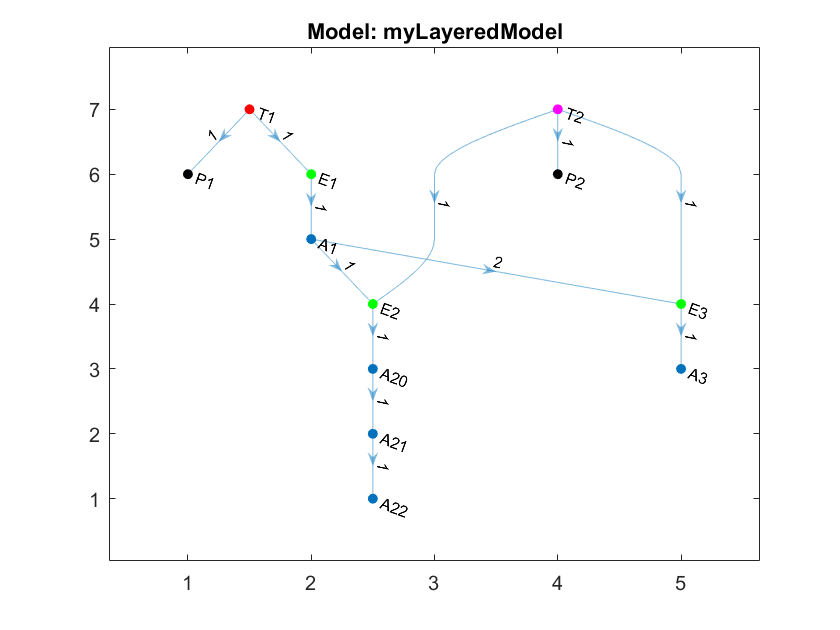
\includegraphics[width=8cm]{./images/lqnView.png}
  \caption{\texttt{LayeredNetwork.plot} method}\label{FIG_lqnView}
\end{figure}
As in the case of the \texttt{Network} class, the \texttt{getGraph} method can be called to inspect the structure of the \texttt{LayeredNetwork} object.

Lastly, the \texttt{jsimgView} and \texttt{jsimwView} methods can be used to visualize in JMT each layer. This can be done by first calling the \texttt{getLayers} method to obtain a cell array consisting of the \texttt{Network} objects, each one corresponding to a layer, and then invoking the \texttt{jsimgView} and \texttt{jsimwView} methods on the desired layer. This is discussed in more details in the next section.

\section{Decomposition into layers}
Layers are a form of decomposition where the influence of resources not explicitly represented in that layer is taken into account through an artificial delay station, placed in a closed loop to the resources~\cite{roli.sevc95}. This artificial delay is used to model the inter-arrival time between calls from resources that belong to other layers.

\subsection{Running a decomposition}
The current version of \textsc{Line} adopts SRVN-type layering~\cite{lqns12}, whereby a layer corresponds to one and only one resource, either a processor or a task. The only exception are reference tasks, which can only appear as clients to their processors.
The \texttt{getLayers} method returns a cell array consisting of the \texttt{Network} objects corresponding to each layer
\begin{lstlisting}
layers = model.getLayers()
\end{lstlisting}
Within each layer, classes are used to model the time a job spends in a given activity or call, with synchronous calls being modeled by classed with label including an arrow, e.g., \texttt{'AS1=>E3'} is a closed class used represent synchronous calls from activity \texttt{AS1} to entry \texttt{E3}. Artificial delays and reference nodes are modelled as a delay station named \texttt{'Clients'}, whereas the task or processor assigned to the layer is modelled as the other node in the layer.

\subsection{Initialization and update}
\label{initialization-and-update}
In general, the parameters of a layer will depend on the steady-state solution of an other layer, causing a cyclic dependence that can be broken only after the model is analyzed by a solver. In order to assign parameters within each layer prior to its solution, the \texttt{LayeredNetwork} class uses the \texttt{initDefault} method, which sets the value of the artificial delay to simple operational analysis bounds~\cite{LazZGS84}.

The layer parameterization depends on a subset of performance indexes stored in a \texttt{param} structure array within the \texttt{LayeredNetwork} class. After initialization, it is possible to update the layer parameterization for example as follows
\begin{lstlisting}
layers = model.getLayers();
for l=1:model.getNumberOfLayers()
    AvgTableByLayer{l} = SolverMVA(layers{l}).getAvgTable;
end
model.updateParam(AvgTableByLayer);
model.refreshLayers;
\end{lstlisting}
Here, the \texttt{refreshParam} method updates the \texttt{param} structure array from a cell array of steady-state solutions for the \texttt{Network} objects in each layer. Subsequently, the \texttt{refreshLayers} method enacts the new parameterization across the \texttt{Network} objects in each layer.

\section{Solvers}
\textsc{Line} offers two solvers for the solution of a \texttt{LayeredNetwork} model consisting in its own native solver (\texttt{LN}) and a wrapper (\texttt{LQNS}) to the LQNS solver~\cite{lqns12}. The latter requires a distribution of LQNS to be available on the operating system command line.

The solution methods available for \texttt{LayeredNetwork} models are similar to those for \texttt{Network} objects. For example, the \texttt{getAvgTable} can be used to obtain a full set of mean performance indexes for the model, e.g.,
\begin{lstlisting}
>> AvgTable = SolverLQNS(model).getAvgTable
AvgTable =
  8x6 table
    Node     NodeType       QLen        Util      RespT      Tput
    ____    ___________    _______    ________    _____    ________
    'P1'    'Processor'        NaN    0.071429     NaN          NaN
    'T1'    'Task'         0.28571    0.071429     NaN     0.071429
    'E1'    'Entry'        0.28571    0.071429       4     0.071429
    'A1'    'Activity'     0.28571    0.071429       4     0.071429
    'P2'    'Processor'        NaN     0.21429     NaN          NaN
    'T2'    'Task'         0.21429     0.21429     NaN      0.21429
    'E2'    'Entry'        0.21429     0.21429       1      0.21429
    'A2'    'Activity'     0.21429     0.21429       1      0.21429
\end{lstlisting}
Note that in the above table, some performance indexes are marked as \texttt{NaN} because they are not defined in a layered queueing network. Further, compared to the \texttt{getAvgTable} method in \texttt{Network} objects, \texttt{LayeredNetwork} do not have an explicit differentiation between stations and classes, since in a layer a task may either act as a server station or a client class.

The main challenge in solving layered queueing networks through analytical methods is that the parameterization of the artificial delays depends on the steady-state performance of the other layers, thus causing a cyclic dependence between input parameters and solutions across the layers. Depending on the solver in use, such issue can be addressed in a different way, but in general a decomposition into layers will remain parametric on a set of response times, throughputs and utilizations.

This issue can be resolved through solvers that, starting from an initial guess, cyclically analyze the layers and update their artificial delays on the basis of the results of these analyses. Both \texttt{LN} and \texttt{LQNS} implement this solution method. Normally, after a number of iterations the model converges to a steady-state solution, where the parameterization of the artificial delays does not change after additional iterations.

\subsection{\texttt{LQNS}}
The LQNS wrapper operates by first transforming the specification into a valid LQNS XML file. Subsequently, LQNS calls the solver and parses the results from disks in order to present them to the user in the appropriate \textsc{Line} tables or vectors. The \texttt{options.method} can be used to configure the LQNS execution as follows:
\begin{itemize}
\item \texttt{options.method='std'} or \texttt{'lqns'}: LQNS analytical solver with default settings.
\item \texttt{options.method='exact'}: the solver will execute the standard LQNS analytical solver with the exact MVA method.
\item \texttt{options.method='srvn'}: LQNS analytical solver with SRVN layering.
\item \texttt{options.method='srvnexact'}: the solver will execute the standard LQNS analytical solver with SRVN layering and  the exact MVA method.
\item \texttt{options.method='lqsim'}: LQSIM simulator, with simulation length specified via the \texttt{samples} field (i.e., with parameter \texttt{-A options.samples, 0.95}).
\end{itemize}

Upon invocation, the \texttt{lqns} or \texttt{lqsim} commands will be searched for in the system path. If they are unavailable, the termination of \texttt{SolverLQNS} will interrupt.

\subsection{\texttt{LN}}
The native \texttt{LN} solver iteratively applies the layer updates until convergence of the steady-state measures. Since updates are parametric on the solution of each layer, \texttt{LN} can apply any of the \texttt{Network} solvers described in the solvers chapter to the analysis of individual layers, as illustrated in the following example for the \texttt{MVA} solver
\begin{lstlisting}
options = SolverLN.defaultOptions;
mvaopt = SolverMVA.defaultOptions;
SolverLN(model, @(layer) SolverMVA(layer, mvaopt), options).getAvgTable
\end{lstlisting}
Options parameters may also be omitted. The \texttt{LN} method converges when the maximum relative change of mean response times across layers from the last iteration is less than \texttt{options.iter\_tol}.

\section{Model import and export}
A \texttt{LayeredNetwork} can be easily read from, or written to, a XML file based on the LQNS meta-model format\footnote{\url{https://raw.githubusercontent.com/layeredqueuing/V5/master/xml/lqn.xsd}}. The read operation can be done using a static method of the \texttt{LayeredNetwork} class, i.e.,
\begin{lstlisting}
model = LayeredNetwork.parseXML(filename)
\end{lstlisting}
Conversely, the write operation is invoked directly on the model object
\begin{lstlisting}
model.writeXML(filename)
\end{lstlisting}
In both examples, \texttt{filename} is a string including both file name and its path.

Finally, we point out that it is possible to export a LQN in the legacy SRVN file format\footnote{\url{http://www.sce.carleton.ca/rads/lqns/lqn-documentation/format.pdf}} by means of the \texttt{writeSRVN(filename)} function.

%\section{Feature comparison}
%
%\begin{table}[thbp]
%\begin{center}
%\begin{tabular}{|c|c|c|}
%\hline
%Feature & LQNS & LN \\
%\hline
%FULL-ACCESS & yes & ? \\
%Device scheduling & FHPS & FRS,... \\
%Task scheduling & FH & FRS,... \\
%Open arrivals & yes & no \\
%MULTI & yes & yes \\
%Infinite servers & yes & yes \\
%SERV-PATTERN & SD & ? \\
%VAR & yes & ? \\
%PAR & yes & no \\
%REPL & yes & ? \\
%ASYNC & yes & no \\
%Forwarding & yes & no \\
%FAST, INTERLOCK & yes & no \\
%\hline
%\end{tabular}
%\end{center}
%\label{TAB_lqn_solver_features}
%\caption{Layered solver features}
%\end{table}


\chapter{Random environments}
\label{Random-environments}
Systems modeled with \textsc{Line} can be described as operating in an environment whose state affects the way the system operates. To distinguish the states of the environment from the ones of the system within it, we shall refer to the former as the environment {\em stages}.  In particular, \textsc{Line} 2.0.0-ALPHA supports the definition of a class of random environments subject to three assumptions:
\begin{itemize}
\item The stage of the environment evolves independently of the state of the system.
\item The dynamics of the environment stage can be described by a continuous-time Markov chain.
\item The topology of the system is independent of the environment stage.
\end{itemize}
The above definitions are in particular appropriate to describe systems whose input parameters change with the environment stage. For example, an environment with two stages, say normal load and peak load, may differ for the number of servers that are available in a queueing station, i.e., the system controller may add more servers during peak load. Upon a stage change in the environment, the model parameters will instantaneously change, but the state reached during the previous stage will be used to initialize the system in the new stage.

Although in a number of cases the system performance may be similar to a weighted combination of the average performance in each stage, this is not true in general, especially if the system dynamic (i.e., the rate at which jobs arrived and get served) and the environment dynamic (i.e., the rate at which the environment changes active stage) happen at similar timescales~\cite{CasTH14}.

\section{Environment object definition}
\label{environment-object-definition}
\subsection{Specifying the environment transitions}
To specify an environment, it is sufficient to define a cell array with entries describing the distribution of time before the environment jumps to a given target state. For example
\begin{lstlisting}
env{1,1} = Exp(0);
env{1,2} = Exp(1);
env{2,1} = Exp(1);
env{2,2} = Exp(0);
\end{lstlisting}
describes an environment consisting of two stage, where the time before a transition to the other stage is exponential with unit rate. If we were to set instead
\begin{lstlisting}
env{2,2} = Erlang.fitMeanAndOrder(1,2);
\end{lstlisting}
this would cause a race condition between two distributions in stage two: the exponential transition back to stage 1, and the Erlang-2 distributed transition with unit rate that remains in stage 2. The latter means that periodically the system will be re-initialized in stage 2, meaning that jobs in execution at a server are required all to restart execution.

In \textsc{Line}, an environment is internally described by a Markov renewal process (MRP) with transition times belonging to the \texttt{PhaseType} class. A MRP is similar to a Markov chain, but state transitions are not restricted to be exponential. Although the time spent in each state of the MRP is not exponential, the MRP can be easily transformed into an equivalent continuous-time Markov chain (CTMC) to enable analysis, a task that \textsc{Line} performs automatically. In the example above, the underpinning CTMC will therefore consider the distribution of the minimum between the exponential and the Erlang-2 distribution, in order to decide the next stage transition.

State space explosion may occur in the definition of an environment if the user specifies a large number of non-exponential transition. For example, a race condition among $n$ Erlang-2 distribution translates at the level of the CTMC into a state space with $2^n$ states. In such situations, it is recommended to replace some of the distributions with exponential ones.

\subsection{Specifying the system models}
\textsc{Line} places loose assumptions in the way the system should be described in each stage. It is just expected that the user supplies a model object, either a \texttt{Network} or a \texttt{LayeredNetwork}, in each stage, and that a transient analysis method is available in the chosen solver, a requirement fulfilled for example by \texttt{SolverFluid}.

However, we note that the model definition can be somewhat simplified if the user describes the system model in a separate MATLAB function, accepting the stage-specific parameters in input to the function. This enables reuse of the system topology across stages, while creating independent model objects. An example of this specification style is given in \texttt{example\_randomEnvironment\_1.m} under \textsc{Line}'s example folder.

\section{Solvers}
The steady-state analysis of a system in a random environment is carried out in \textsc{Line} using the blending method~\cite{CasTH14}, which is an iterative algorithm leveraging the transient solution of the model. In essence, the model looks at the \emph{average} state of the system at the instant of each stage transition, and upon restarting the system in the new stage re-initializes it from this average value. This algorithm is implemented  in \textsc{Line} by the \texttt{SolverEnv} class, which is described next.

\subsection{\texttt{ENV}}
 The \texttt{SolverEnv} class applies the blending algorithm by iteratively carrying out a transient analysis of each system model in each environment stage, and probabilistically weighting the solution to extract the steady-state behavior of the system.

 As in the transient analysis of \texttt{Network} objects, \textsc{Line} does not supply a method to obtain mean response times, since Little's law does not hold in the transient regime. To obtain the mean queue-length, utilization and throughput of the system one can call as usual the \texttt{getAvg} method on the \texttt{SolverEnv} object, e.g.,
\begin{lstlisting}
models = {model1, model2, model3, model4};
envSolver = SolverEnv(models, env, @SolverFluid,options);
[QN,UN,TN] = envSolver.getAvg()
\end{lstlisting}
Note that as model complexity grows, the number of iterations required by the blending algorithm to converge may grow large. In such cases, the \texttt{options.iter\_max} option may be used to bound the maximum analysis time. 

\clearpage
\bibliographystyle{IEEEtran}
\bibliography{LINE}
\appendix

\chapter{Examples}
\label{Examples}
%In this chapter, we report code of the \textsc{Line} examples under the \texttt{examples} folder and their outputs.
In this appendix, we summarize the features demonstrated in the \textsc{Line} scripts that are available under the \texttt{examples} folder.

{
\begin{table}[thbp]
\footnotesize
\renewcommand{\arraystretch}{1.2}
\centering
\caption{Examples}
\begin{tabular}{|l|l|}
\hline
\textbf{Example} & \textbf{Problem}\\
\hline
\texttt{example\_cdfRespT\_1} &  Station response time distribution in a single-class single-job closed network\\
\texttt{example\_cdfRespT\_2} &  Station response time distribution in a multi-chain closed network\\
\texttt{example\_cdfRespT\_3} &  Station response time distribution in a multi-chain open network\\
\texttt{example\_cdfRespT\_4} &  Simulation-based station response time distribution analysis\\
\texttt{example\_cdfRespT\_5} &  Station response time distribution under increasing job populations\\
\hline
\texttt{example\_closedModel\_1} &  Solving a single-class exponential closed queueing network\\
\texttt{example\_closedModel\_2} &  Solving a closed queueing network with a multi-class FCFS station\\
\texttt{example\_closedModel\_3} &  Solving exactly a multi-chain product-form closed queueing network\\
\texttt{example\_closedModel\_4} &  Local state space generation for a station in a closed network\\
\texttt{example\_closedModel\_5} &  1-line exact MVA solution of a cyclic network of PS and INF stations\\
\texttt{example\_closedModel\_6} &  Closed network with round robin scheduling\\
\hline
\texttt{example\_initState\_1} &  Specifying an initial state and prior in a single class model.\\
\texttt{example\_initState\_2} &  Specifying an initial state and prior in a multiclass model.\\
\hline
\texttt{example\_layeredModel\_1} & Analyze a layered network specified in a LQNS XML file \\
\texttt{example\_layeredModel\_2} & Specifying and solving a basic layered network\\
\hline
\texttt{example\_misc\_1} &  Use of performance indexes handles\\
\texttt{example\_misc\_2} &  Update and refresh of service times\\
\texttt{example\_misc\_3} &  Parameterization of a discriminatory processor sharing (DPS) station\\
\texttt{example\_misc\_4} &  Automatic detection of solvers that cannot analyze the model\\
\hline
\texttt{example\_mixedModel\_1} & Solving a queueing network model with both closed and open classes \\
\hline
\texttt{example\_openModel\_1} & Solving a queueing network model with open classes, scalar cutoff options \\
\texttt{example\_openModel\_2} & 1-line solution of a tandem network of PS and INF stations\\
\texttt{example\_openModel\_3} & Solving a queueing network model with open classes, matrix cutoff options \\
\texttt{example\_openModel\_4} & Trace-driven simulation of an M/M/1 queue\\
\hline
\texttt{example\_randomEnvironment\_1} &  Solving a model in a 2-stage random environment \\
\texttt{example\_randomEnvironment\_2} &  Solving a model in a 4-stage random environment \\
\hline
\texttt{example\_stateProbabilities\_1} &  Computing marginal state probabilities for a node\\
\texttt{example\_stateProbabilities\_2} &  Computing marginal state probabilities for a node under class-switching\\
\texttt{example\_stateProbabilities\_3} &  Computing joint state probabilities for the system\\
\hline
\end{tabular}
\label{TAB_examples_closedModel}
\end{table}
}

%\subsection{\texttt{example\_closedModel\_1.m}}
%\paragraph{Code.} This example illustrates the definition in \textsc{Line} of a single-class closed queueing network with two nodes,a  delay and a processor sharing queue, and probabilistic routing. All available \textsc{Line} solvers are instantiated and run on the model.
%%\lstinputlisting[language=matlab,numbers=left,linerange=1-27]{examples/example_closedModel_1.m}
%
%\lstset{
%    language=matlab,
%    tabsize=3,
%    frame=single,
%    basicstyle=\ttfamily\scriptsize,
%    %caption=Test,
%    label=code:sample,
%    frame=shadowbox,
%    rulesepcolor=\color{gray},
%    xleftmargin=20pt,
%    framexleftmargin=15pt,
%    keywordstyle=\color{black},
%    commentstyle=\color{magenta},
%    stringstyle=\color{red},
%    %numbers=left,
%    %numberstyle=\tiny,
%    %numbersep=5pt,
%    aboveskip=10pt,
%    breaklines=true,
%    showstringspaces=false,
%    emph={environment,stage,envParameter,coxDistribution,coxParameter},
%    emphstyle={\color{blue}}}
%
%\begin{lstlisting}
%clear;
%model = Network('model');
%
%node{1} = Delay(model, 'Delay');
%node{2} = Queue(model, 'Queue1', SchedStrategy.PS);
%jobclass{1} = ClosedClass(model, 'Class1', 5, node{1}, 0);
%
%node{1}.setService(jobclass{1}, Exp.fitMeanAndSCV(1.0)); % mean = 1
%node{2}.setService(jobclass{1}, Exp.fitMeanAndSCV(2.0)); % mean = 2
%
%model.addLink(node{1}, node{1});
%model.addLink(node{1}, node{2});
%model.addLink(node{2}, node{1});
%model.addLink(node{2}, node{2});
%
%node{1}.setProbRouting(jobclass{1}, node{1}, 0.7)
%node{1}.setProbRouting(jobclass{1}, node{2}, 0.3)
%node{2}.setProbRouting(jobclass{1}, node{1}, 1.0)
%
%solver = {};
%solver{end+1} = SolverCTMC(model);
%solver{end+1} = SolverJMT(model);
%solver{end+1} = SolverSSA(model);
%solver{end+1} = SolverFluid(model);
%solver{end+1} = SolverMVA(model);
%solver{end+1} = SolverNC(model);
%for s=1:length(solver)
%    fprintf(1,'SOLVER: %s\n',solver{s}.getName());
%    AvgTable = solver{s}.getAvgTable()
%end
%\end{lstlisting}
%
%\paragraph{Output.} The output of the previous script is as follows. Small approximation errors and simulation sampling error are responsible from small deviations from the exact values, which are those reported by the CTMC solver. The error of the simulation solvers (JMT, SSA) can be increase with larger \texttt{options.samples} values.
%
%\begin{lstlisting}
%SOLVER: SolverCTMC
%AvgTable =
%  2x6 table
%    Station         Class          QLen      Util      RespT      Tput
%    ________    ______________    ______    _______    ______    ______
%    'Delay'     'Class1'    1.6327     1.6327         1    1.6327
%    'Queue1'    'Class1'    3.3673    0.97961    6.8748    0.4898
%SOLVER: SolverJMT
%AvgTable =
%  2x6 table
%    Station         Class          QLen      Util      RespT      Tput
%    ________    ______________    ______    _______    ______    _______
%    'Delay'     'Class1'    1.5491     1.5491    1.0042     1.6093
%    'Queue1'    'Class1'      3.39    0.98315     6.967    0.48154
%SOLVER: SolverSSA
%AvgTable =
%  2x6 table
%    Station         Class          QLen      Util      RespT      Tput
%    ________    ______________    ______    _______    ______    _______
%    'Delay'     'Class1'    1.6309     1.6309         1     1.6309
%    'Queue1'    'Class1'    3.3691    0.97853    6.8694    0.49045
%SOLVER: SolverFluid
%AvgTable =
%  2x6 table
%    Station      Class       QLen      Util     RespT      Tput
%    ________    ________    ______    ______    ______    ______
%    'Delay'     'Class1'    1.6667    1.6667         1    1.6667
%    'Queue1'    'Class1'    3.3333         1    6.6667       0.5
%SOLVER: SolverMVA
%AvgTable =
%  2x6 table
%    Station         Class          QLen      Util      RespT      Tput
%    ________    ______________    ______    _______    ______    _______
%    'Delay'     'Class1'    1.5314     1.5314         1     1.5314
%    'Queue1'    'Class1'    3.4686    0.91886    7.5497    0.45943
%SOLVER: SolverNC
%AvgTable =
%  2x6 table
%    Station         Class          QLen      Util      RespT      Tput
%    ________    ______________    ______    _______    ______    ______
%    'Delay'     'Class1'    1.6327     1.6327         1    1.6327
%    'Queue1'    'Class1'    3.3673    0.97961    6.8748    0.4898
%\end{lstlisting}
%
%\subsection{\texttt{example\_closedModel\_2.m}}
%\paragraph{Code.}  This model shows an example of 2-class, 1-chain, closed queueing network with non-exponential service processes.
%\begin{lstlisting}
%model = Network('model');
%
%node{1} = Delay(model, 'Delay');
%node{2} = Queue(model, 'Queue1', SchedStrategy.FCFS);
%node{2}.setNumServers(2);
%
%jobclass{1} = ClosedClass(model, 'Class1', 2, node{1}, 0);
%jobclass{2} = ClosedClass(model, 'Class2', 2, node{1}, 0);
%
%node{1}.setService(jobclass{1}, Erlang(3,2));
%node{1}.setService(jobclass{2}, HyperExp(0.5,3.0,10.0));
%
%node{2}.setService(jobclass{1}, HyperExp(0.1,1.0,10.0));
%node{2}.setService(jobclass{2}, Exp(1));
%
%M = model.getNumberOfStations();
%K = model.getNumberOfClasses();
%
%P = cell(K,K);
%P{1,1} = [0.3,0.1; 0.2,0];
%P{1,2} = [0.6,0; 0.8,0];
%P{2,2} = [0,1; 0,0];
%P{2,1} = [0,0; 1,0];
%
%model.link(P);
%
%options = Solver.defaultOptions;
%options.keep=true;
%options.verbose=1;
%options.samples=5e3;
%
%solver={};
%solver{end+1} = SolverCTMC(model,options);
%solver{end+1} = SolverJMT(model,options);
%solver{end+1} = SolverSSA(model,options);
%solver{end+1} = SolverFluid(model,options);
%solver{end+1} = SolverMVA(model,options);
%solver{end+1} = SolverNC(model,options);
%for s=1:length(solver)
%    fprintf(1,'SOLVER: %s\n',solver{s}.getName());
%    AvgTable = solver{s}.getAvgTable()
%end
%\end{lstlisting}
%\paragraph{Output.}
%\begin{lstlisting}
%SOLVER: SolverCTMC
%CTMC generator and state space saved in: C:\X\AppData\Local\Temp\tp49e94d44_0a44_4d6f_ac03_68e9bb550698.mat
%CTMC analysis completed in 0.940576 sec
%AvgTable =
%  4x6 table
%    Station         Class          QLen        Util       RespT      Tput
%    ________    ______________    _______    ________    _______    _______
%    'Delay'     'Class1'     1.5404      1.5404    0.66667     2.3107
%    'Delay'     'Class2'    0.34044     0.34044    0.21667     1.5712
%    'Queue1'    'Class1'    0.11129    0.021951    0.48165    0.23107
%    'Queue1'    'Class2'     2.0078     0.78562     1.2779     1.5712
%SOLVER: SolverJMT
%JMT Model: C:\X\AppData\Local\Temp\jsimg\tpf370d5af_7e96_4aca_bf73_0cf3c496ad2c.jsimg
%JMT Command: java -cp "C:\X\Dropbox\code\line-solver.git\bin\line\src\solvers\JMT\JMT.jar" jmt.commandline.Jmt sim "C:\X\AppData\Local\Temp\jsimg\tpf370d5af_7e96_4aca_bf73_0cf3c496ad2c.jsimg" -seed 23000 --illegal-access=permit
%JMT analysis completed in 17.300090 sec
%AvgTable =
%  4x6 table
%    Station         Class          QLen        Util       RespT      Tput
%    ________    ______________    _______    ________    _______    _______
%    'Delay'     'Class1'     1.6167      1.6167    0.65263     2.3886
%    'Delay'     'Class2'     0.3398      0.3398     0.2185     1.6104
%    'Queue1'    'Class1'    0.10854    0.018798    0.47573    0.23014
%    'Queue1'    'Class2'     1.9709     0.79182     1.2305     1.6049
%SOLVER: SolverSSA
%SSA samples:   5000
%SSA analysis completed in 19.095364 sec
%AvgTable =
%  4x6 table
%    Station         Class          QLen        Util       RespT      Tput
%    ________    ______________    _______    ________    _______    ______
%    'Delay'     'Class1'     1.5162      1.5162    0.64725    2.3425
%    'Delay'     'Class2'    0.32429     0.32429     0.2142     1.514
%    'Queue1'    'Class1'    0.09591    0.022254     0.4954    0.1936
%    'Queue1'    'Class2'     2.0636     0.75698     1.2922     1.597
%SOLVER: SolverFluid
%Fluid analysis completed in 0.144978 sec [21 iterations]
%AvgTable =
%  4x6 table
%    Station         Class           QLen        Util       RespT      Tput
%    ________    ______________    ________    ________    _______    _______
%    'Delay'     'Class1'      1.7625      1.7625    0.66667     2.6438
%    'Delay'     'Class2'     0.38951     0.38951    0.21667     1.7978
%    'Queue1'    'Class1'    0.050231    0.025116       0.19    0.26438
%    'Queue1'    'Class2'      1.7978     0.89888          1     1.7978
%SOLVER: SolverMVA
%MVA analysis completed in 0.051836 sec
%AvgTable =
%  4x6 table
%    Station         Class           QLen        Util       RespT      Tput
%    ________    ______________    ________    ________    _______    _______
%    'Delay'     'Class1'      1.5557      1.5557    0.66667     2.3336
%    'Delay'     'Class2'     0.34382     0.34382    0.21667     1.5868
%    'Queue1'    'Class1'    0.057094    0.022169    0.24466    0.23336
%    'Queue1'    'Class2'      2.0434     0.79342     1.2877     1.5868
%SOLVER: SolverNC
%NC analysis completed in 0.002516 sec
%AvgTable =
%  4x6 table
%    Station      Class        QLen       Util       RespT      Tput
%    ________    _________    _______    _______    _______    _______
%    'Delay'     'Class1'     1.0825     1.0825    0.66667     1.6237
%    'Delay'     'Class2'    0.23922    0.23922    0.21667     1.1041
%    'Queue1'    'Class1'    0.34337    0.12016     2.1148    0.16237
%    'Queue1'    'Class2'     2.3349    0.81706     2.1148     1.1041
%\end{lstlisting}
%
%\subsection{\texttt{example\_closedModel\_3.m}}
%\paragraph{Code.} This model shows an example of 3-class, 2-chain, closed queueing network with non-exponential service processes.
%\begin{lstlisting}
%model = Network('model');
%
%node{1} = Delay(model, 'Delay');
%node{2} = Queue(model, 'Queue1', SchedStrategy.PS);
%
%jobclass{1} = ClosedClass(model, 'Class1', 2, node{1}, 0);
%jobclass{2} = ClosedClass(model, 'Class2', 0, node{1}, 0);
%jobclass{3} = ClosedClass(model, 'Class3', 1, node{1}, 0);
%
%node{1}.setService(jobclass{1}, Erlang(3,2));
%node{1}.setService(jobclass{2}, HyperExp(0.5,3.0,10.0));
%node{1}.setService(jobclass{3}, Exp(1));
%
%node{2}.setService(jobclass{1}, HyperExp(0.1,1.0,10.0));
%node{2}.setService(jobclass{2}, Exp(2));
%node{2}.setService(jobclass{3}, Exp(3));
%
%M = model.getNumberOfStations();
%K = model.getNumberOfClasses();
%
%P = cell(K,K);
%
%P{1,1} = [0.3,0.1; 0.2,0];
%P{1,2} = [0.6,0; 0.8,0];
%P{1,3} = zeros(M);
%
%P{2,1} = [0,0; 1,0];
%P{2,2} = [0,1; 0,0];
%P{2,3} = zeros(M);
%
%P{3,1} = zeros(M);
%P{3,2} = zeros(M);
%P{3,3} = circul(M);
%
%model.link(P);
%
%options = Solver.defaultOptions;
%options.keep=true;
%options.verbose=1;
%
%solver={};
%solver{end+1} = SolverCTMC(model,options);
%solver{end+1} = SolverFluid(model,options);
%solver{end+1} = SolverMVA(model,options);
%solver{end+1} = SolverNC(model,options);
%for s=1:length(solver)
%    fprintf(1,'SOLVER: %s\n',solver{s}.getName());
%    AvgTable = solver{s}.getAvgTable()
%    AvgChainTable = solver{s}.getAvgChainTable()
%    AvgSysChainTable = solver{s}.getAvgSysTable()
%end
%\end{lstlisting}
%\paragraph{Output.} This is the output on screen of this example.
%\begin{lstlisting}
%SOLVER: SolverCTMC
%CTMC generator and state space saved in: C:\X\AppData\Local\Temp\tpafad0e65_193e_4a46_a779_b2ac27a9f97f.mat
%CTMC analysis completed in 0.168026 sec
%AvgTable =
%  6x6 table
%    Station         Class     QLen        Util       RespT      Tput
%    ________    _________    ________    ________    _______    _______
%    'Delay'     'Class1'     0.94598     0.94598    0.66667      1.419
%    'Delay'     'Class2'     0.20906     0.20906    0.21667     0.9649
%    'Delay'     'Class3'     0.63412     0.63412          1    0.63412
%    'Queue1'    'Class1'    0.044719    0.026961    0.31515     0.1419
%    'Queue1'    'Class2'     0.80023     0.48245    0.82934     0.9649
%    'Queue1'    'Class3'     0.36588     0.21137    0.57699    0.63412
%AvgChainTable =
%  4x7 table
%    Station      Chain       Classes       QLen       Util       RespT      Tput
%    ________    ________    __________    _______    _______    _______    _______
%    'Delay'     'Chain1'    {1x2 cell}      1.155      1.155    0.48452     2.3839
%    'Delay'     'Chain2'    {1x1 cell}    0.63412    0.63412          1    0.63412
%    'Queue1'    'Chain1'    {1x2 cell}    0.84495    0.50941    0.35444     1.1068
%    'Queue1'    'Chain2'    {1x1 cell}    0.36588    0.21137    0.57699    0.63412
%AvgSysChainTable =
%  2x4 table
%     Chain       Classes      SysRespT    SysTput
%    ________    __________    ________    _______
%    'Chain1'    {1x2 cell}    0.83897      2.3839
%    'Chain2'    {1x1 cell}      1.577     0.63412
%SOLVER: SolverFluid
%Fluid analysis completed in 0.059826 sec [1 iterations]
%AvgTable =
%  6x6 table
%    Station         Class     QLen        Util       RespT      Tput
%    ________    ________    ________    ________    _______    ______
%    'Delay'     'Class1'      1.1367      1.1367    0.66667     1.705
%    'Delay'     'Class2'     0.25121     0.25121    0.21667    1.1594
%    'Delay'     'Class3'        0.75        0.75          1      0.75
%    'Queue1'    'Class1'    0.032396    0.032396       0.19    0.1705
%    'Queue1'    'Class2'     0.57971     0.57971        0.5    1.1594
%    'Queue1'    'Class3'        0.25        0.25    0.33333      0.75
%AvgChainTable =
%  4x7 table
%    Station      Chain       Classes       QLen       Util       RespT      Tput
%    ________    ________    __________    _______    _______    _______    ______
%    'Delay'     'Chain1'    {1x2 cell}     1.3879     1.3879    0.48452    2.8645
%    'Delay'     'Chain2'    {1x1 cell}       0.75       0.75          1      0.75
%    'Queue1'    'Chain1'    {1x2 cell}    0.61211    0.61211    0.21369    1.3299
%    'Queue1'    'Chain2'    {1x1 cell}       0.25       0.25    0.33333      0.75
%AvgSysChainTable =
%  2x4 table
%     Chain       Classes      SysRespT    SysTput
%    ________    __________    ________    _______
%    'Chain1'    {1x2 cell}    0.69821     2.8645
%    'Chain2'    {1x1 cell}     1.3333       0.75
%SOLVER: SolverMVA
%MVA analysis completed in 0.029756 sec
%AvgTable =
%  6x6 table
%    Station      Class       QLen        Util       RespT      Tput
%    ________    _________   ________    ________    _______    _______
%    'Delay'     'Class1'     0.90548     0.90548    0.66667     1.3582
%    'Delay'     'Class2'     0.20011     0.20011    0.21667    0.92359
%    'Delay'     'Class3'     0.61295     0.61295          1    0.61295
%    'Queue1'    'Class1'    0.047336    0.025806    0.34851    0.13582
%    'Queue1'    'Class2'     0.84707      0.4618    0.91714    0.92359
%    'Queue1'    'Class3'     0.38705     0.20432    0.63147    0.61295
%AvgChainTable =
%  4x7 table
%    Station      Chain       Classes       QLen       Util       RespT      Tput
%    ________    ________    __________    _______    _______    _______    _______
%    'Delay'     'Chain1'    {1x2 cell}     1.1056     1.1056    0.48452     2.2818
%    'Delay'     'Chain2'    {1x1 cell}    0.61295    0.61295          1    0.61295
%    'Queue1'    'Chain1'    {1x2 cell}     0.8944     0.4876    0.39197     1.0594
%    'Queue1'    'Chain2'    {1x1 cell}    0.38705    0.20432    0.63147    0.61295
%AvgSysChainTable =
%  2x4 table
%     Chain       Classes      SysRespT    SysTput
%    ________    __________    ________    _______
%    'Chain1'    {1x2 cell}    0.87649      2.2818
%    'Chain2'    {1x1 cell}     1.6315     0.61295
%SOLVER: SolverNC
%NC analysis completed in 0.044545 sec
%AvgTable =
%  6x6 table
%    Station      Class        QLen       Util        RespT       Tput
%    ________    ________    ________    _______    _________    _______
%    'Delay'     'Class1'      252.34     252.34      0.66667     378.51
%    'Delay'     'Class2'      55.766     55.766      0.21667     257.38
%    'Delay'     'Class3'     0.63412    0.63412            1    0.63412
%    'Queue1'    'Class1'    0.044719     7.1916    0.0011815     37.851
%    'Queue1'    'Class2'     0.80023     128.69    0.0031091     257.38
%    'Queue1'    'Class3'     0.36588    0.21137      0.57699    0.63412
%AvgChainTable =
%  4x7 table
%    Station      Chain       Classes       QLen       Util        RespT       Tput
%    ________    ________    __________    _______    _______    _________    _______
%    'Delay'     'Chain1'    {1x2 cell}      308.1      308.1      0.48452     635.89
%    'Delay'     'Chain2'    {1x1 cell}    0.63412    0.63412            1    0.63412
%    'Queue1'    'Chain1'    {1x2 cell}    0.84495     135.88    0.0013288     295.23
%    'Queue1'    'Chain2'    {1x1 cell}    0.36588    0.21137      0.57699    0.63412
%AvgSysChainTable =
%  2x4 table
%     Chain       Classes      SysRespT     SysTput
%    ________    __________    _________    _______
%    'Chain1'    {1x2 cell}    0.0031452     635.89
%    'Chain2'    {1x1 cell}        1.577    0.63412
%\end{lstlisting}


\end{document} 